\chapter{Introduction}
The Lead Radius Experiment-II (PREX-II) and the Calcium Radius Experiment (CREX) are 
high-precision experiments that measure the tiny parity-violating (PV) asymmetry,
at parts-per-million (ppm) level, of longitudinally polarized electrons scattered 
off neutron-rich targets (\Pb and \Ca), from which the weak form factor, weak
charge and neutron distribution, and finally the
neutron skin thickness of the target nucleus, will be extracted.

The PV asymmetry ($\CA_{\text{PV}}$) comes from the interference between the 
electromagnetic (EM) and neutral weak one-boson exchange amplitudes, because weak 
interaction doesn't conserve parity. Since the EM 
interaction has been well understood, the PV asymmetry measurement allows 
us to derive the weak charge and therefore the neutron (which has almost all the 
weak charge) distribution inside a nucleus.

Parity-violating electron scattering (PVES) experiments require % medium to high energy and 
an electron beam with a high longitudinal polarization, which, for PREX-II and CREX,
was provided by the  Continuous Electron Beam Accelerator Facility (CEBAF) 
at Thomas Jefferson National Accelerator Facility (TJNAF, also known as JLab). 
The excellent beam qualities and dedicated instrumentation at JLab allowed 
the asymmetry measurements to be statistics-limited.

% physical implication
% 1. neutron distribution
%%%%%%%%%%%%%%%%%%%%%%%%%%%%%%%%%%%%%%%%%%%%%%%%%%%%%%%%%%%%%%%%%%%%%%%%
\section{Point-Neutron Radius and Neutron Skin}
Despite the development of modern physics, we don't have a clear way to 
compute the size of a nucleus, and maybe we don't even know what we mean 
when we say that.
% More precisely, we don't have a complete and thorough understanding of nuclei. 
In a simple picture, one may estimate the nuclear radius as $R = R_0 A^{1/3}$, 
where $A$ is the nuclear mass number 
and $R_0$ is an approximately constant coefficient that can be experimentally 
identified ($R_0 \approx 1.20$~fm \cite{ROYER2008105}). However, this simple 
picture only works for spherical nuclei, it fails for deformed nuclei.
It is better to calculate the radius of a nucleus from its nucleon density
distribution.
Physicists have calculated and precisely measured the point-proton (charge) radius of many nuclei,
but neutron, due to its neutrality, remains a stubborn obstacle in 
our measurements of the inner structure of nuclei. Especially for heavy nuclei,
where more neutrons than protons are needed to bound the nuclei, it is neutron
radius rather than proton radius that defines the size of a heavy nucleus.

When we talk about the proton or neutron radius, it is a concept under the
framework of Quantum Mechanics (QM), rather than the classical radius of an object.
In QM, a particle is represented by a wave function, 
whose magnitude is related to the probability of finding this particle in a specific
state, so the neutron (proton) Root-Mean-Square (RMS) radius is defined as:
% why RMS radius, rather than r\rho(r) directly?
\begin{equation}
    R_{p, n} \equiv \langle R_{p,n}^2\rangle^{1/2} = \sqrt{\frac{\int d^3\vec{r}\,r^2\,\rho_{p,n}(\vec{r})}{\int d^3\vec{r}\,\rho_{p,n}(\vec{r})}}
    \label{eq:nucleon_rms_radius}
\end{equation}
where $\rho(\vec{r})$ is the normalized proton (neutron) density at position $\vec{r}$.
\begin{equation}
    \int d^3\vec{r} \rho_{p, n}(\vec{r}) = 1 
\end{equation}

There are numerous papers in literature reporting high-precision  
(with an uncertainty at $0.01$~fm level)
measurement of the proton (charge) radius ($R_p$) of various nuclei through atomic 
and nuclear experiments \cite{DEVRIES1987495, ANGELI201369}. In contrast, there
are few precise determinations of the neutron radius ($R_n$). The difficulty is that
the neutron carries no electric charge, so one can measure its size through only 
strong or weak interaction. Both methods suffer from their own limitations. 

The weak interaction is so weak ($\alpha_W = 10^{-6}$) that it is hard to control 
systematic uncertainties if measured directly.
% , compared to the background EM interaction ($\alpha = 1/137$), 
Hence people turn to measurement of the PV asymmetry. By taking the asymmetry
between two electron beams with opposite helicities, many systematic uncertainties
are cancelled, therefore high precision can be achieved.

In terms of the strong interaction, the effective coupling has large theoretical uncertainties rooted 
in the non-perturbative nature of the underlying Quantum Chromodynamics (QCD) at low energy scale, 
and the interpretation of hadronic measurement is usually model dependent. 

Despite all these challenges, there has been a lot of effort and progress from the community 
to explore different aspects of neutron radius (and neutron skin thickness): 
the hadronic probes include pion \cite{ALLARDYCE19731}, proton \cite{LOMBARDI1972103,PhysRevC.82.044611}, 
antiproton \cite{PhysRevC.76.014311} and alpha particle \cite{KRASZNAHORKAY2004224};
atomic experiments like electric dipole polarizabilities \cite{Roca_Maza_2012} and 
pygmy dipole resonances \cite{PhysRevC.88.044610}
also provide inputs to our understanding.
Experimentally, with model dependence, the current measures of $R_n$ have a resolution of better than 1\%.
On the theory side, the most precise estimate of $R_n$ appears to come from nuclear models
that have been constrained primarily by data other than measurements	% FIXME reference
of neutron radii. Therefore, a precise measurement of $R_n$ will provide a powerful 
independent check of the basic nuclear theory.
\begin{comment}
% https://doi.org/10.1016/j.nuclphysa.2003.11.034
\item proton
    \begin{itemize}
	\item high-energy polarized proton
	\item Relativistic Impulse Approximation (RIA) with free nucleon-nucleon interaction
    \end{itemize}
\item pion
    \begin{itemize}
	\item in the $\Delta(1332)$ region, $\pi^- N$ interaction is 3 times larger than $\pi^- p$.
	\item strong absorption at the surface, sensitive to the tail of neutron distributions;
	    increase pion energy to reduce xsection
	\item applicable to only light stable nuclei
    \end{itemize}
\item antiproton
    \begin{itemize}
	\item slow antiproton capture (like an electron)
    \end{itemize}
\item PVES
\item GDR: Giant Dipole Resonance
\item SDR: Spin-Dipole Resonance
\end{comment}

Experimentally, the nucleon radius is measured from its corresponding form
factors (FFs). According to QM, under the Born approximation, the matrix element (ME) 
for the scattering of a plane wave (a free particle) from a Coulomb-like potential 
(a target nucleus) is:
\begin{equation}
    \begin{aligned}
	\CM_{fi} &= \bra{\Psi_f}V(\vec{r})\ket{\Psi_i} 
		= \int e^{-i\vec{p}_f\vec{r}}V(\vec{r}) e^{i\vec{p}_i\vec{r}} d^3\vec{r}    \\	% 1
	    &= \int e^{i(\vec{p_i} - \vec{p_f})\vec{r}} d^3\vec{r} 
		\int \frac{Q_t\rho(\vec{r'})}{4\pi|\vec{r} - \vec{r'}|} d^3\vec{r'} \\	% 2
	    &= \int \int e^{i\vec{q} \vec{r} } 
		 \frac{Q_t \rho(\vec{r'})}{4\pi|\vec{r} - \vec{r'}|} d^3\vec{r} d^3\vec{r'} \\	% 2
	    &= \int\int e^{i\vec{q}(\vec{r} - \vec{r'})} 
		\frac{Q_t\rho(\vec{r'})}{4\pi|\vec{r} - \vec{r'}|} e^{i\vec{q}\vec{r'}} d^3\vec{r} d^3\vec{r'}   \\  % 3
	    &= \int e^{i\vec{q}\vec{R}} \frac{Q_t}{4\pi|\vec{R}|} d^3\vec{R} 
		\int \rho(\vec{r'}) e^{i\vec{q} \vec{r'}}d^3 \vec{r'}	\\  % 4
	    &= (\CM_{fi})_{\text{Mott}} F(\vec{q})   \\	% 5
    \end{aligned}
    \label{eq:ME}
\end{equation}
where $\vec{p}_i$ ($\vec{p}_f$) denotes momentum of the incoming (outgoing) particle,
$\vec{q} = \vec{p}_i - \vec{p}_f$ refers to the momentum transfer during the scattering
and $Q_t$ is the total charge of the target nucleus. The ME can be factorized into two parts.
The amplitude of a Mott scattering, which is the scattering of a particle from 
a point-like nucleus with charge $Q_t$ and a modification
due to the inner structure of the target nucleus, which is called the FF:
\begin{equation}
    F(\vec{q}) = \int \rho(\vec{r}) e^{i\vec{q} \vec{r}} d^3\vec{r}
    \label{eq:ff}
\end{equation}
The FF is just the Fourier transform of the spatial density distribution.
Conversely, once the FFs at different $\vec{q}$ are known (measured) , one can
derive the charge distribution:
\begin{equation}
    \rho(\vec{r}) = \int F(\vec{q}) e^{-i\vec{q}\vec{r}} d^3\vec{q}
\end{equation}
What's more, $F(\vec{q})$ is experimentally measurable, as shown in Eq.~\ref{eq:ME}:
\begin{equation}
    F(\vec{q}) = \frac{\CM_{fi}}{(\CM_{fi})_{\text{Mott}}} 
	= \sqrt{\frac{\sigma_{\text{measured}}}{\sigma_{\text{Mott}}}} 
\end{equation}
The problem is, experimentally, there is no way to cover the whole phase space 
of $\vec{q}$; we can measure only limited data points at selected $\vec{q}$ values. 
Therefore, some phenomenological models are needed to extract the charge density distribution. 
% FIXME: examples of phenomenological models

For a spherically symmetric density distribution, 
$\rho(\vec{r}) = \rho({|\vec{r}|}) = \rho(r)$, 
one can calculate the corresponding FF as:
\begin{equation}
    F(\vec{q}) = \int \rho(r) e^{iqr\cos\theta} 2\pi r^2 \sin\theta dr d\theta
	= 4\pi \int r \rho(r) \frac{\sin{(qr)}}{q} dr
    \label{eq:spherically_symmetric_FF}
\end{equation}
One can see that for a Coulomb-like potential, $F(\vec{q})$ doesn't depend on
the direction of $\vec{q}$, but only on its magnitude: $q$. For the convenience 
of Lorentz Invariance, $F$ is usually written in terms of $Q^2 = -q^2$, rather
than $q$, so we will use $F(q^2)$ or $F(Q^2)$ hereafter.

Some typical spherically symmetric density distributions and their 
corresponding FFs are shown in Fig.~\ref{fig:FFs}.
\begin{figure}[!h]
    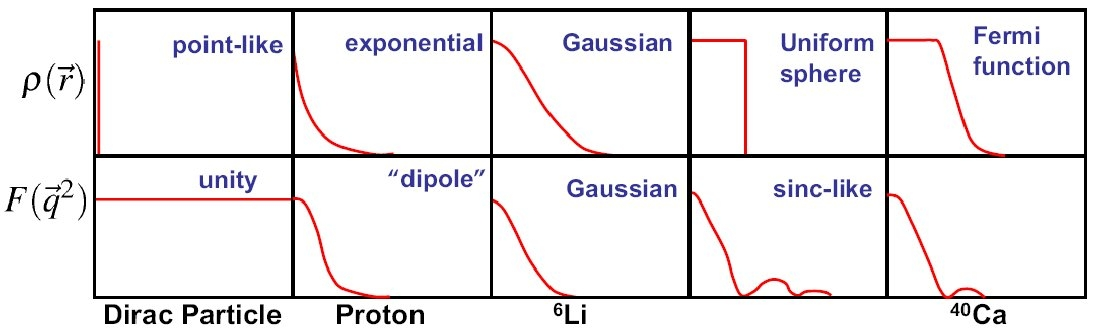
\includegraphics[width=0.9\linewidth]{rho_vs_FF}
    \caption{Characteristic of FFs w.r.t. different density distribution functions}
    \label{fig:FFs}
\end{figure}

In the small $\vec{q}^2$ limit ($q^2 << 1$), one can do the Fourier expansion on both
sides of Eq.~\ref{eq:spherically_symmetric_FF}:
\begin{equation}
    F(q^2) = F(0) + \left.\frac{dF}{dq^2}\right|_{q^2=0} \times q^2 + \cdots	\\
    \label{eq:FF_FE_1}
\end{equation}
\begin{equation}
    \begin{aligned}
	F(q^2) &= 4\pi \int r \rho(r) \frac{\sin{(qr)}}{q} dr \\
	    &= 4\pi \int \rho(r) r \left( r - \frac{1}{6} q^2r^3 + \cdots \right) dr	\\
	    &= \int \rho(r)  \left( 1 - \frac{1}{6} q^2r^2 + \cdots \right) 4\pi r^2 dr	\\
	    &= 1 - \frac{1}{6}q^2\langle R^2 \rangle + \cdots \\
    \end{aligned}
    \label{eq:FF_FE_2}
\end{equation}
Matching Eq.~\ref{eq:FF_FE_1} to \ref{eq:FF_FE_2} yields
\begin{equation}
    \langle R^2 \rangle = \int r^2 \rho(r) d^3\vec{r} = -6 \left. \frac{dF(q^2)}{dq^2} \right|_{q^2 = 0}
\end{equation}
This equation prompts how to measure a RMS radius:
one can measure the FFs at some small $q^2$ points, extrapolate them 
to $q^2 = 0$, then the slope at $q^2 = 0$ will be the RMS radius.
\footnote{This is why we use the RMS radius rather than the more physical definition of: 
$\langle R \rangle = \int  r \rho(\vec{r}) d^3\vec{r}$.}

For charged proton, the FF will be the precisely measured EM FF:
\begin{equation}
    \langle R_p^2 \rangle \approx \langle R_{ch}^2 \rangle= -6 \left. \frac{dF_{EM}(q^2)}{dq^2} \right|_{q^2 = 0}
\end{equation}
Since neutron is neutral, its RMS radius will be measured from its weak charge FF:
\begin{equation}
    \langle R_n^2 \rangle \approx \langle R_W^2 \rangle = -6 \left. \frac{dF_{W}(q^2)}{dq^2} \right|_{q^2 = 0}
\end{equation}
The difference between these RMS radii is called the neutron skin thickness:
\begin{equation}
    R_{\text{skin}} = R_n - R_p = \sqrt{\langle R_n^2 \rangle} - \sqrt{\langle R_p^2 \rangle}
\end{equation}
a concept that was first suggested by Johnson and Teller \cite{PhysRev.93.357}
and first observed in the $K^-$ meson capture processes \cite{BURHOP1969625}.

The neutron skin is founded in neutron-rich atomic nuclei that have more 
neutrons than protons. Analog to the atomic electron shell model, the nuclear
shell model proposes that protons and neutrons also arrange themselves in
shells from low to high energy, without disturbing each other.
The higher the energy level, the larger the orbit radius.
For symmetric nuclei, we expect similar neutron radii to proton radii. 
For neutron-rich nuclei, the extra neutrons
have to stay on higher energy orbits after filling all low energy ones, forming
a larger radius than proton and therefore the neutron skin.

The deep reason for these extra neutrons form a neutron skin instead of
a neutron core is the symmetry energy and its dependence on density. 
Symmetry energy represents the penalty for breaking the proton-neutron symmetry,
whose value is positively related to density \cite{10.3389/fphy.2019.00213}.
The core area has a higher nucleon density than the surface, the higher the density, 
the larger the symmetry energy, therefore the lower the binding energy 
\footnote{the energy needed to break down a bounded nuclear system: $BE(N, Z) = M(N, Z)c^2 - Zm_p c^2 - Nm_n c^2$}, 
the less stable the nuclei. So it is the symmetry energy that pushes these extra neutrons to 
the surface. On the other hand, the more nucleons on the surface, the stronger 
the surface tension, so the surface tension favors squeezing extra neutrons % FIXME reference for the surface tension
into the core. The balance between the symmetry energy and 
the surface tension determine the thickness of the neutron skin.

% FIXME: a conclusion paragraph stating the importance of the measurement

%%%%%%%%%%%%%%%%%%%%%%%%%%%%%%%%%%%%%%%%%%%%%%%
\subsection{Theoretical Models} 
\label{subsec:models}
Though we don't know the actual neutron distribution, one would not expect too
much difference between the proton and neutron distributions, even in nuclei with
asymmetric numbers of protons and neutrons. So the proton distribution is a good
starting point for the study of neutron distribution, given that we have quite
good knowledge about proton distribution, learned from various eA and AA scatterings. 
The elastic scattering cross section is:
\begin{equation}
    \frac{d\sigma}{d\Omega} = \left( \frac{d\sigma}{d\Omega} \right)_{\text{Mott}} |F(q^2)|^2
\end{equation}

The FF encodes information about the charge structure of a nucleus. It is an interference
effect, finite size of the scattering center introduces a phase difference between
different plane waves scattered from different points in space.
\begin{figure}
    \centering
    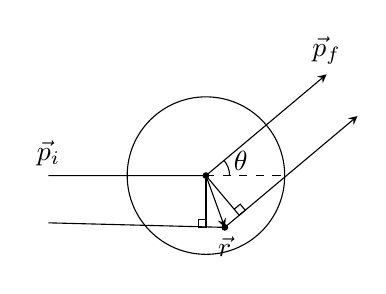
\begin{tikzpicture}
	% theta = 40, r = 0.7
	\coordinate (O) at (0, 0);
	\coordinate (P) at (-70:0.7);
	\draw (O) circle (1 cm);
	\draw[fill=black] (O) circle (1 pt);
	\draw[fill=black] (P) circle (1 pt);
	\draw[-stealth] (-2, 0) node [above] {$\vec{p}_i$} -- (O) -- ++(40:2) node [above, sloped] {$\vec{p}_f$};
	\draw[-stealth] (-2, -0.6) -- (P) -- ++(40:2.2);
	\draw[-stealth] (O) -- (P) node[below] {$\vec{r}$};
	\draw[dashed] (O) -- +(1, 0);
	\draw (0.3, 0) arc (0:40:0.3) node[right] {$\theta$};

	\draw (O) -- ++(0, -0.657785) -- ++(-0.1, 0) -- ++(0, 0.1) -- ++(0.1, 0);
	\draw (O) -- ++(-50:0.657785) -- ++(40:0.1) -- ++(130:0.1) -- ++(-140:0.1);
    \end{tikzpicture}
    \caption[eA scattering]{Schematic plot of eA scattering. As one can see, the wave scattered
    at position $\vec{r}$ will travel extra distance compared to the one scattered
    at the object center, which leads to a phase difference of:
    $\delta = e^{i[\vec{p}_i \cdot \vec{r} + (-\vec{p}_f) \cdot \vec{r}]} = e^{i\vec{q}\cdot\vec{r}}$.
    }
    \label{fig:FF_phase_diff}
\end{figure}

Consider a simple hard ball model:
\begin{equation}
    \rho(r) = 
    \begin{cases}
	\frac{3}{4\pi R^3}  & r \le R	\\
	0		    & r > R   \\
    \end{cases}
    \label{eq:hard_ball_model}
\end{equation}
Then the FF will be:
\begin{equation}
    F(q^2) = \frac{3}{(qR)^3} \left( \sin(qR) - qR\cos(qR) \right)
\end{equation}
where $q = 2p\sin(\theta/2)$.

Given the Mott cross section: % FIXME: citation
% \begin{equation}
%     \left( \frac{d\sigma}{d\Omega} \right)_{Mott} = 
%     \begin{cases}
% 	\frac{Z^2 \alpha^2}{4E^2\sin^4(\theta/2)}\cos^2(\theta/2)   
% 	    & \text{light nuclei} \ Z\alpha << 1  \\
% 	\frac{Z^2 \alpha^2}{4E^2\sin^4(\theta/2)}\cos^2(\theta/2) \left[ 1 + \pi Z \alpha \frac{\sin(\theta/2)(1-\sin(\theta/2)))}{\cos^2(\theta/2)}\right]   
% 	    & \text{medium nuclei}  \\
%     \end{cases}
% \end{equation}
\begin{equation}
    \left( \frac{d\sigma}{d\Omega} \right)_{\text{Mott}} = 
	\frac{Z^2 \alpha^2}{4E^2\sin^4(\theta/2)}\cos^2(\theta/2)   
\end{equation}
the resulting cross section, as a function of the scattering angle, is shown in Fig.~\ref{fig:ca_xsec}.
\begin{figure}
    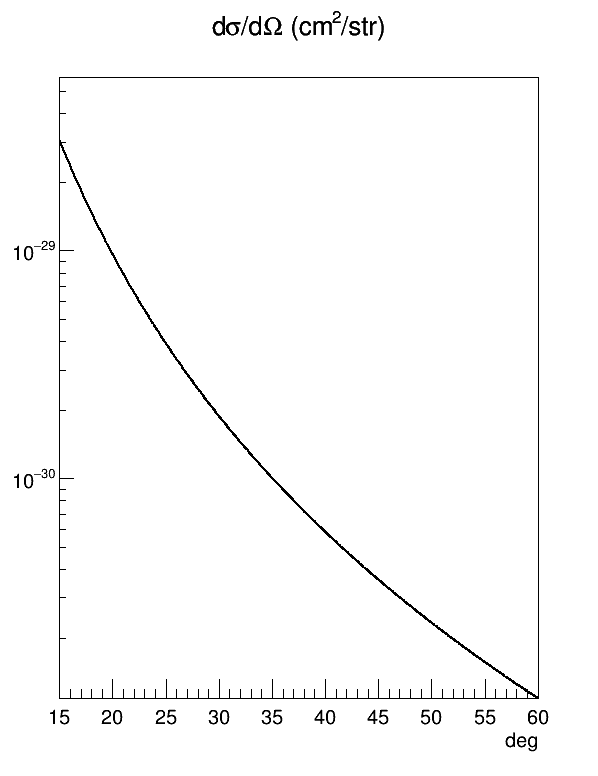
\includegraphics[width=0.32\linewidth]{ca48_xsec_mott}
    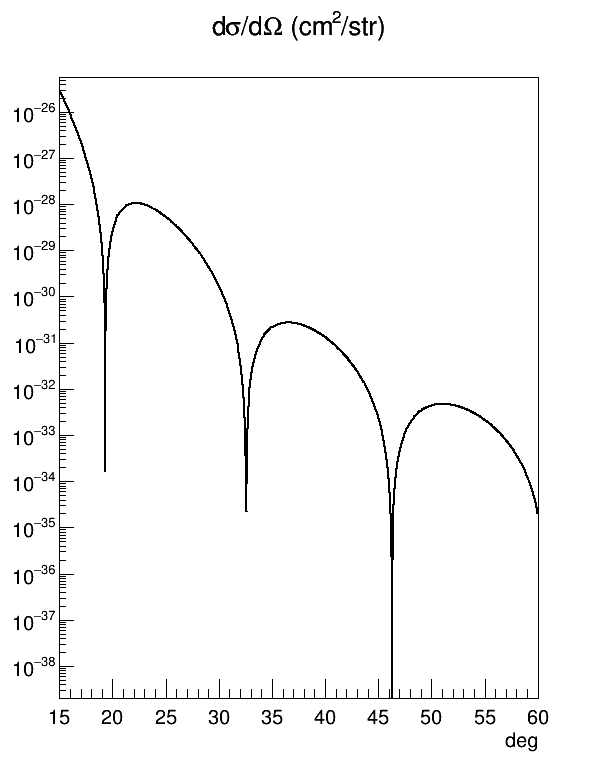
\includegraphics[width=0.32\linewidth]{ca48_xsec_hard_ball}
    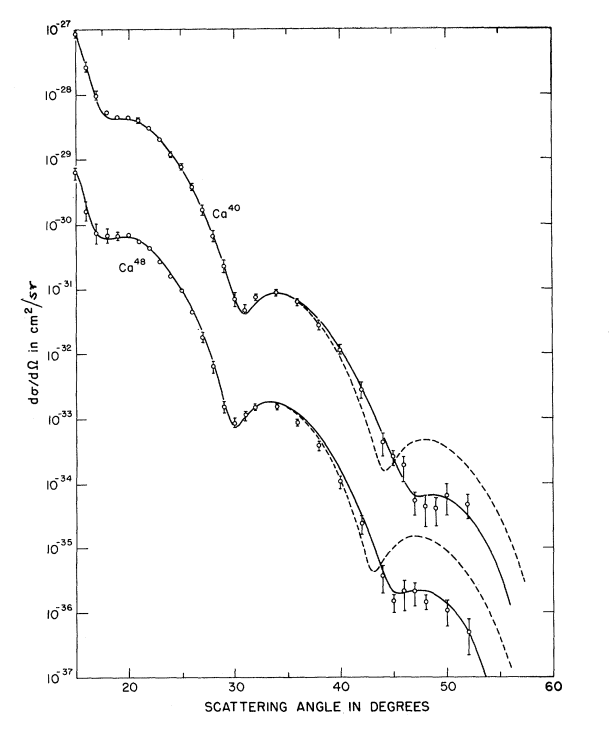
\includegraphics[width=0.32\linewidth]{ca_xsec_exp}
    \caption[xsection of \Ca]{Left: Mott cross section of electron elastically scattered off a \Ca
    target. Parameters: $p=E=757.5$~MeV.
    Middle: cross section of electron elastically scattered off Ca48 with the hard ball
    model (\ref{eq:hard_ball_model}). Parameters: $E =  757.5$~MeV, $R=A^{1/3}$~fm. 
    Right: experimental values (dots) and theoretical prediction (solid line).
    The theoretical calculation assumes the charge distribution as a three-parameter Fermi function (\ref{eq:3-para_Fermi}).
    The \Ca \ (\ca) cross sections are multiplied by $10^{-1}$ ($10$) to separate them
    \cite{PhysRevLett.19.527}. A similar cross section plot of \Pb can be found
    in \cite{PhysRevLett.38.152}.
    }
    \label{fig:ca_xsec}
\end{figure}

While the hard ball model doesn't reproduce the experimental distribution, it does
characterize the real distribution and show how the FF modifies the cross section:
the oscillating dips. A more realistic model of the density distribution is the
Saxon-Woods distribution (also called the Fermi two-parameter model or the Fermi
distribution):
\begin{equation}
    \rho(r) = \frac{\rho(0)}{1 + \exp((r-R)/t)}
\end{equation}
where $R = (1.2A^{1/3} - 0.48)$~fm denotes the nuclear force radius at which 
$\rho(r) = \frac{\rho(0)}{2}$,
and $t \sim 0.4-0.5$~fm for  $A > 40$ indicates the surface thickness, 
over which $\rho(r)$ falls from 90\% to 10\%.
\begin{figure}[!h]
    \centering
    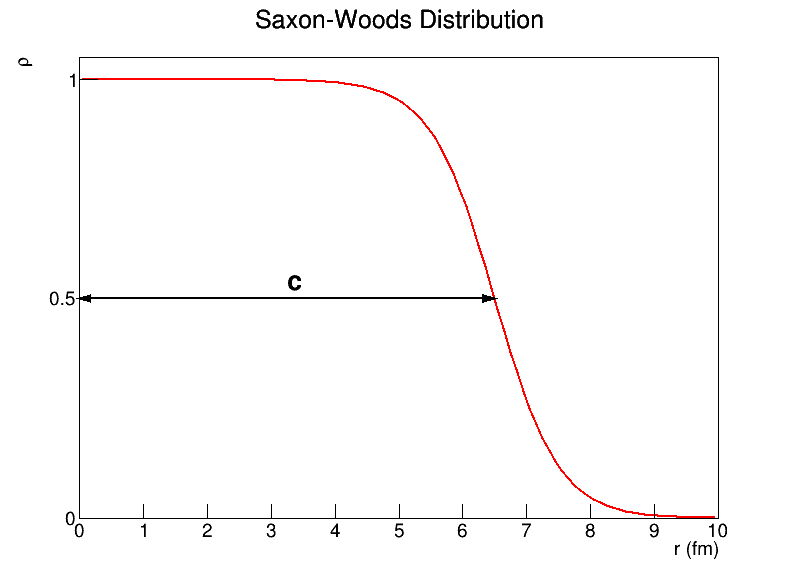
\includegraphics[width=0.5\linewidth]{fermi_distribution}
    \caption[fermi distribution]
    {In the nuclear Shell Model, it is assumed that nucleons occupy 
    different eigenstates of the same spherically symmetric average potential.
    This potential, unlike that in atomic shell model, needed to be guessed. 
    It turns out that the Saxon-Woods model is a good candidate: 
    $V(r) = -\frac{V(0)}{1+\exp((r-c)/a)}$ ($c$ is the half-height radius and $a$ represents
    diffuseness of the distribution). This potential is formed
    by all other nucleons, so it is approximately proportional to the nucleon density, 
    therefore the same distribution for nucleon density.} 
\end{figure}

Fig.~\ref{fig:ca_xsec} (right) uses a fine tuned three-parameter Fermi function:
\begin{equation}
    \rho(r) = \frac{\rho_0(1 + \omega r^2/R^2)}{1 + \exp((r-R)/t)}
    \label{eq:3-para_Fermi}
\end{equation}
the central depression parameter $\omega$ allows the central density to be depressed
or raised, depending on the sign of $\omega$. More detailed discussion about the Fermi 
distribution can be found in \cite{Maximon:1966sqn}.

One example model based on the Fermi distribution is the FSUGold \cite{PhysRevLett.95.122501},
the neutron distribution of \Pb predicted by FSUGold is shown in Fig.~\ref{fig:FSUGold_pb208}.
\begin{figure}[!h]
    \centering
    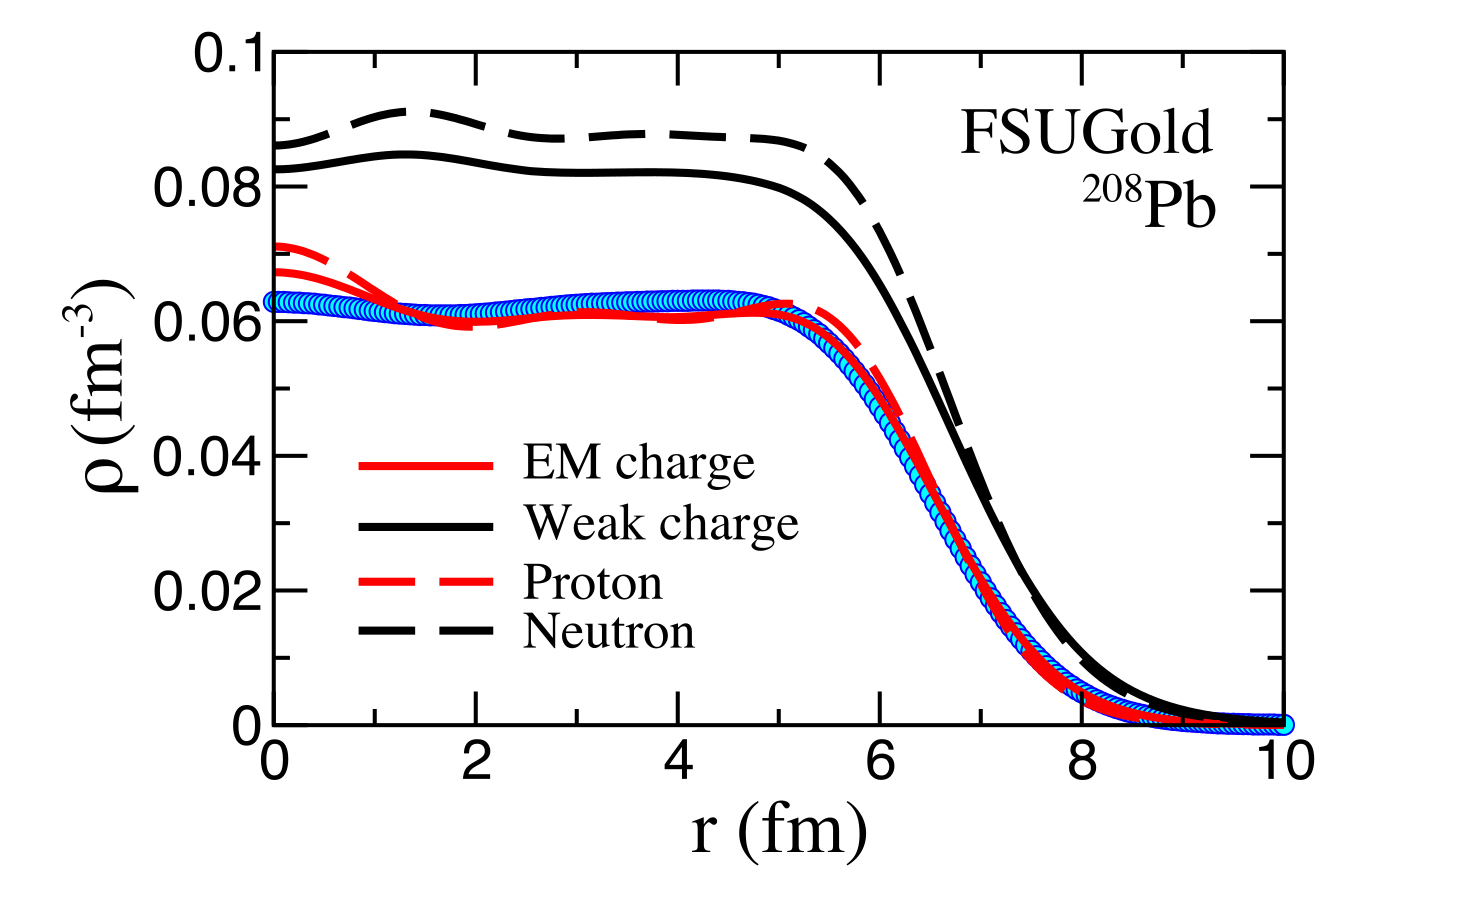
\includegraphics[width=0.6\linewidth]{FSUGold_pb208}
    \caption[Neutron distribution from FSUGold]
    {Neutron and weak charge distribution in \Pb predicted by the FSUGold model.
    The blue dots are experimental measurements of the charge distribution.}
    \label{fig:FSUGold_pb208}
\end{figure}

For medium and heavy nuclei, the Born approximation,
where the incoming and outgoing waves are treated as plane waves,
doesn't hold. 
In reality, the waves are distorted by the intense nuclear EM field, making them
no longer plane waves. We have to take into account the 
Coulomb distortion effect, which will modify the PV asymmetry significantly.
Coulomb distortion can be understood as multiple EM interactions with
the same nucleus, so the distortion correction is proportional to $Z\alpha$. 
Obviously, this correction is more important for \Pb than for light and medium
nuclei, because of its large Z value.
Coulomb-distortion could reduce the PV asymmetry by as much as 30\% as shown 
in Fig.~\ref{fig:diff_by_Coulomb_distortion}.
\begin{figure}[H]
    \centering
    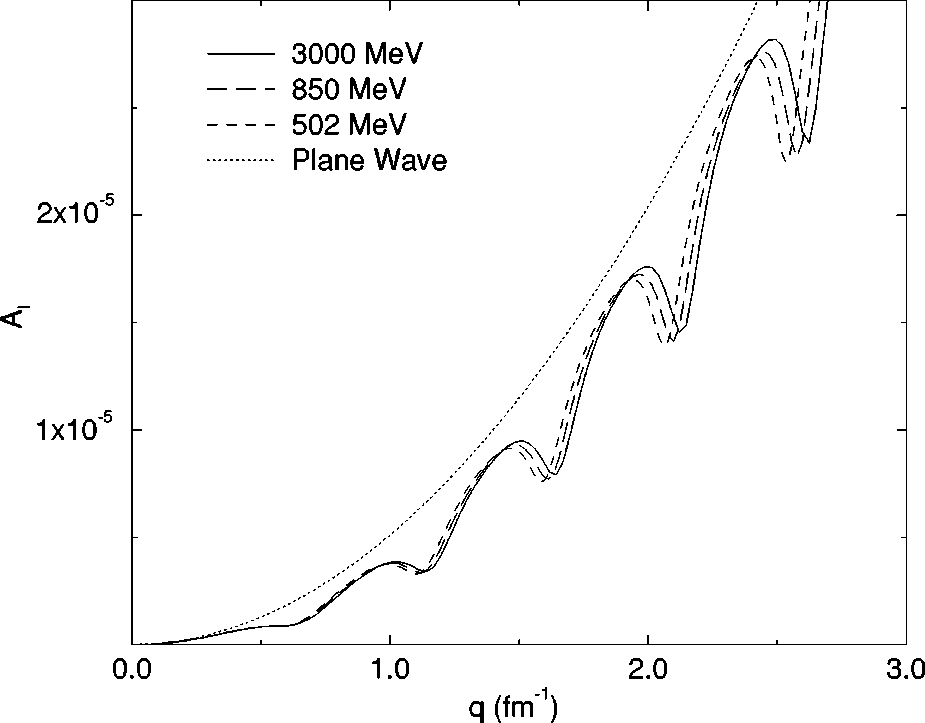
\includegraphics[width=0.5\linewidth]{Coulomb_distortion_Pb208_diff}
    \caption[Coulomb distortion]
    {Comparison of PV asymmetries with and without the effect of Coulomb
    distortion for \Pb. The calculation assumes the same weak and charge densities,
    which are taken to be the three-parameter Fermi function \cite{PhysRevC.57.3430}.
    }
    \label{fig:diff_by_Coulomb_distortion}
\end{figure}

With these information, one is able to solve the Dirac equation directly to know
the PV asymmetry, as shown in Fig.~\ref{fig:Coulomb_distortion}.

\begin{figure}[!h]
    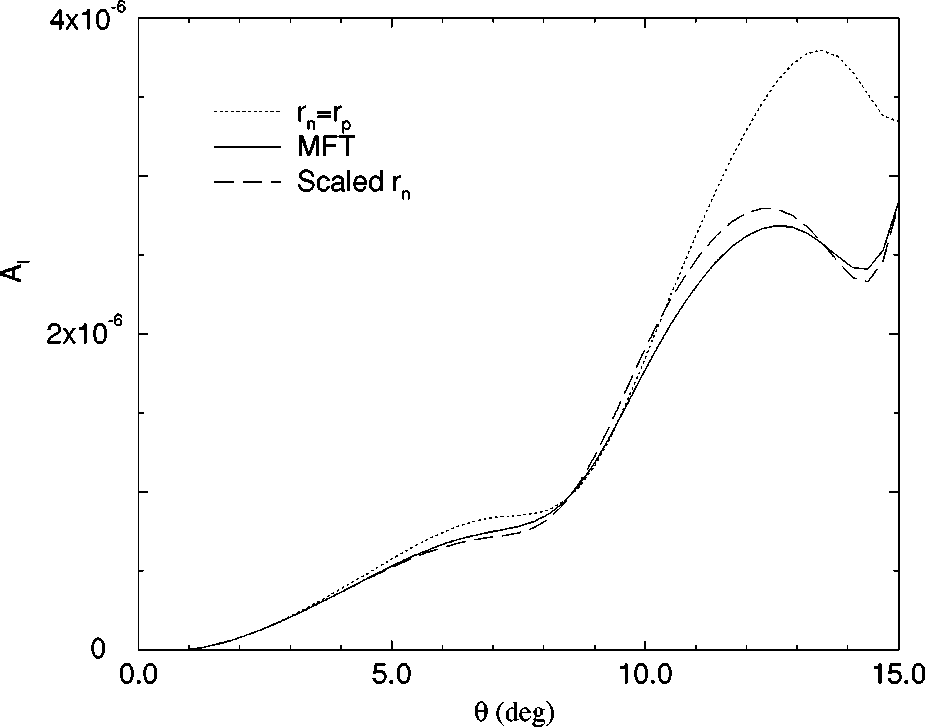
\includegraphics[width=0.49\linewidth]{Coulomb_distortion_Pb208}
    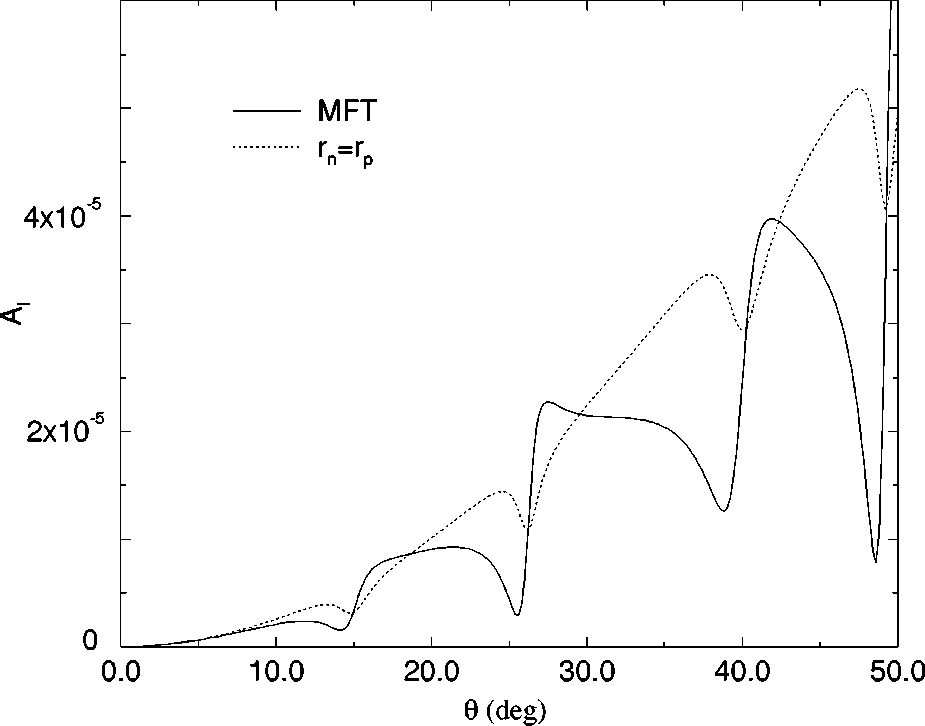
\includegraphics[width=0.48\linewidth]{Coulomb_distortion_Ca48}
    \caption[PV asymmetry for \Pb and \Ca]
    {PV asymmetry for \Pb (left) and \Ca (right) versus scattering angle 
    at 850~MeV (Coulomb distortion correction included). 
    The dotted curve assumes the same weak and charge distributions (three-parameter Fermi function), 
    while the solid curve is based on relativistic mean field densities (MFT).
    The dashed curve uses a stretched density distribution based on the three-parameter Fermi function \cite{PhysRevC.57.3430}.
    }
    \label{fig:Coulomb_distortion}
\end{figure}

% 2. symmetry energy dependence on density
%%%%%%%%%%%%%%%%%%%%%%%%%%%%%%%%%%%%%%%%%%%%%%%%%%%%%%%%%%%%%%%%%%%%%%%%
\section{Symmetry Energy} 
The binding energy of a nuclear system depends on both the total number of nucleons ($A$),
and the difference between numbers of protons and neutrons.
Using the liquid drop model (LDM), we get the Bethe-Weizsacker Semi-empirical Mass Formula:
\begin{equation}
    \begin{gathered}
	E\ (\mathrm{MeV}) = \textcolor{black}{a_V A} 
	    - \textcolor{blue}{a_S A^{2/3}} 
	    - \textcolor{green}{a_C\frac{Z(Z-1)}{A^{1/3}}} 
	    - \textcolor{red}{a_A\frac{(N-Z)^2}{A}} 
	    + \textcolor{cyan}{\delta a_p A^{-3/4}} \\
	\delta a_p A^{-3/4} = 
	    \begin{cases}
		+a_p A^{-3/4}	& \text{Z, N even} \\
		0		& \text{A odd}	\\
		-a_p A^{-3/4}	& \text{Z, N odd (A even)} \\
	    \end{cases}
    \end{gathered}
    \label{eq:mass-formula}
\end{equation}

\begin{itemize}
    % https://en.wikipedia.org/wiki/Semi-empirical_mass_formula
    \color{black} \item Volume term ($a_V$): strong force between nearby nucleons ($a_V \sim 16$~MeV)
    \color{blue}  \item Surface term ($a_S$): correction to the volume term ($a_S \sim 18$~MeV)
    \color{green} \item Coulomb term ($a_C$): repulsion due to EM charge ($a_C \sim 0.7$~MeV)
    \color{red}   \item Asymmetry term ($a_A$): correction from the Pauli exclusion principle ($a_A \sim 24$~MeV)
    \color{cyan}  \item Pairing term ($\delta$): correction caused by the spin coupling effect 
	($a_p \sim 34$~MeV)
\end{itemize}

The first three terms are natural:
the volume term reflects the short-range nature of the strong interaction; the
surface term comes from the fact that nucleons on the surface aren't completely 
surrounded by other nucleons; and the Coulomb term reveals the EM interactions between
protons. 

The asymmetry term may not be so obvious. It is based solely on the Pauli exclusion principle. % FIXME reference for Pauli exclusion principle
In heavy nuclei,
more neutrons than protons are needed to balance the repulsion between protons.
Due to the Pauli exclusion principle, the energy of these extra neutrons will be 
higher than the rest nucleons, therefore introducing this correction term.

The pairing term is a small correction due to nuclei's preference for `paired spin'. % FIXME is there a reference for this
Nuclei with even numbers of proton (Z) and neutron (N) are more stable than those with odd number
of Z and N.

Regarding the nuclear system as a free Fermi gas of protons and neutrons, the 
kinetic energy ($E_k$) of this system will be:
\begin{equation}
    E_k = E_N + E_Z = \frac{3}{5}ZE_F^p + \frac{3}{5}NE_F^n
\end{equation}
Since the Fermi energy is proportional to $n^{2/3}$, $E_k$ can be written as:
\begin{equation}
    E_k = C(Z^{5/3} + N^{5/3})
\end{equation}
where $C$ is a constant coefficient. 
Expand it in terms of $N-Z$ (see appendix \ref{ap:symmetry_energy}), we will get:
\begin{equation}
    \begin{aligned}
	E_k &= 2^{-2/3}C\left(A^{5/3} + \frac{5}{9}\frac{(N-Z)^2}{A^{1/3}} \right) + O((N-Z)^4) \\
	    &= \frac{3}{5} E_F A + \frac{1}{3}E_F\frac{(N-Z)^2}{A} + O((N-Z)^4) \\
    \end{aligned}
    \label{eq:free_fermi_gas}
\end{equation}
The first term in Eq.~\ref{eq:free_fermi_gas} contributes to the volume term 
of the binding energy and the second term is minus the 
asymmetry term because $E_k$ contributes to the binding energy negatively.

For a general discussion, we can ignore the Coulomb term in Eq.~\ref{eq:mass-formula}
to focus on the homogeneous nuclear (residual strong) interaction between nucleons, 
and the pairing term which is too small.
So, instead of true nuclei, the object of discussion is extended to any nuclear 
system composed of Z charge-less protons and N neutrons. Now the equation
of state (EOS) for nuclear matter is simplified.
\begin{equation}
    \begin{aligned}
	E &= a_V A - a_S A^{2/3} - a_A\frac{(N-Z)^2}{A}  \\
	e &= \frac{E}{A} = a_V - a_S A^{-1/3} - a_A\frac{(N-Z)^2}{A^2}
    \end{aligned}
    \label{eq:modified-mass-formula-1}
\end{equation}

We can also discard the surface term in Eq.~\ref{eq:modified-mass-formula-1}. 
Obviously, we can't guarantee
any specific shape of the nuclear system; what's more, for the most common limit
-- the infinite nuclear system, we don't need to consider the surface 
term at all, because an infinite system has no surface. By neglecting the surface
term, we write:
\begin{equation}
    \begin{aligned}
	E &= a_V A - a_A\frac{(N-Z)^2}{A}  \\
	e &= \frac{E}{A} = a_V - a_A\frac{(N-Z)^2}{A^2} = e_0(A) - a_A\beta^2 
    \end{aligned}
    \label{eq:modified-mass-formula-2}
\end{equation}
Here $\beta = \frac{N-Z}{N+Z}$ is defined as asymmetry between the number of neutrons and protons,
which is called the isospin asymmetry.

For an infinite system, density, instead of $A$, will be a better choice to parameterize
the EOS. So we replace $N$, $Z$ and $A$ with their corresponding density: $\rho_n$, 
$\rho_p$ and $\rho$ ($\beta = \frac{\rho_n - \rho_p}{\rho}$). Similarly, $E$ is replaced by
its density counterpart $e$.
Therefore we are considering an infinite uniform nuclear system at 0 temperature that interacts
only via the nuclear force. For any identified $\rho$,
Eq.~\ref{eq:modified-mass-formula-2} will be:
\begin{equation}
    e(\rho, \beta) = e(\rho, 0) + S(\rho)\beta^2 + O(\beta^4)
    \label{eq:symmetry-energy}
    % e(\rho, 0) = 31.7~MeV; L \sim 60~MeV
\end{equation}
where $S(\rho)$ is a density dependent coefficient.

This is an expansion of the binding energy per nucleon around $\beta = 0$.
Due to the isospin symmetry between proton and neutron, any isoscalar quantities
$F$ will remain unchanged under $n \leftrightarrow p$ interchange, while isovector 
quantities $G$ will change sign. $\beta$ is an isovector, so for a smooth $F(\beta)$,
its expansion around $\beta = 0$ has even terms only:
$$ F(\beta) = F_0 + F_2\beta^2 + F_4\beta^4 + \dots $$
On the other hand, for a smooth $G(\beta)$, its expansion around $\beta = 0$ has
odd terms only:
$$ G(\beta) = G_1\beta + G_3\beta^3 + \dots $$

$e$ is an isoscalar, it doesn't change under $n \leftrightarrow p$ interchange 
as one can see from Eq.~\ref{eq:modified-mass-formula-2}. The coefficient 
$S(\rho) = \frac{\partial^2 e (\rho, \beta)}{\partial \beta^2}$ is
what we call the symmetry energy, a key parameter in describing a wide
range of nuclear properties and phenomena. It describes how much energy would be
released when exchanging all protons into neutrons for a symmetric nuclear system. 
% a plot for symmetry energy from some models

Not only is $S$ itself important, but also its dependence on $\rho$. 
By convention, $S(\rho)$ is expanded around the nuclear saturation density $\rho_0$
(following the free Fermi gas assumption):
\begin{equation}
    S(\rho) = S(\rho_0) 
    + \left.\frac{dS}{d\rho}\right|_{\rho_0}(\rho - \rho_0)
    + \frac{1}{2}\left.\frac{d^2S}{d\rho^2}\right|_{\rho_0}(\rho - \rho_0)^2
    + \frac{1}{6}\left.\frac{d^3S}{d\rho^3}\right|_{\rho_0}(\rho - \rho_0)^3
    + \dots
\end{equation}
From which, we have some auxiliary parameters defined:
\begin{equation}
    \begin{aligned}
	S_0 &= S(\rho_0)	\\
	L   &= 3\rho_0\left.\frac{dS}{d\rho}\right|_{\rho_0}	\\
	K_{\text{sym}}	&= 9\rho_0^2\left.\frac{d^2S}{d\rho^2}\right|_{\rho_0}	\\
	Q_{\text{sym}}	&= 27\rho_0^3\left.\frac{d^3S}{d\rho^3}\right|_{\rho_0}	\\
    \end{aligned}
\end{equation}
Among them, $L$ represents $S$'s dependence on $\rho$.
\begin{figure}[!h]
    \centering
    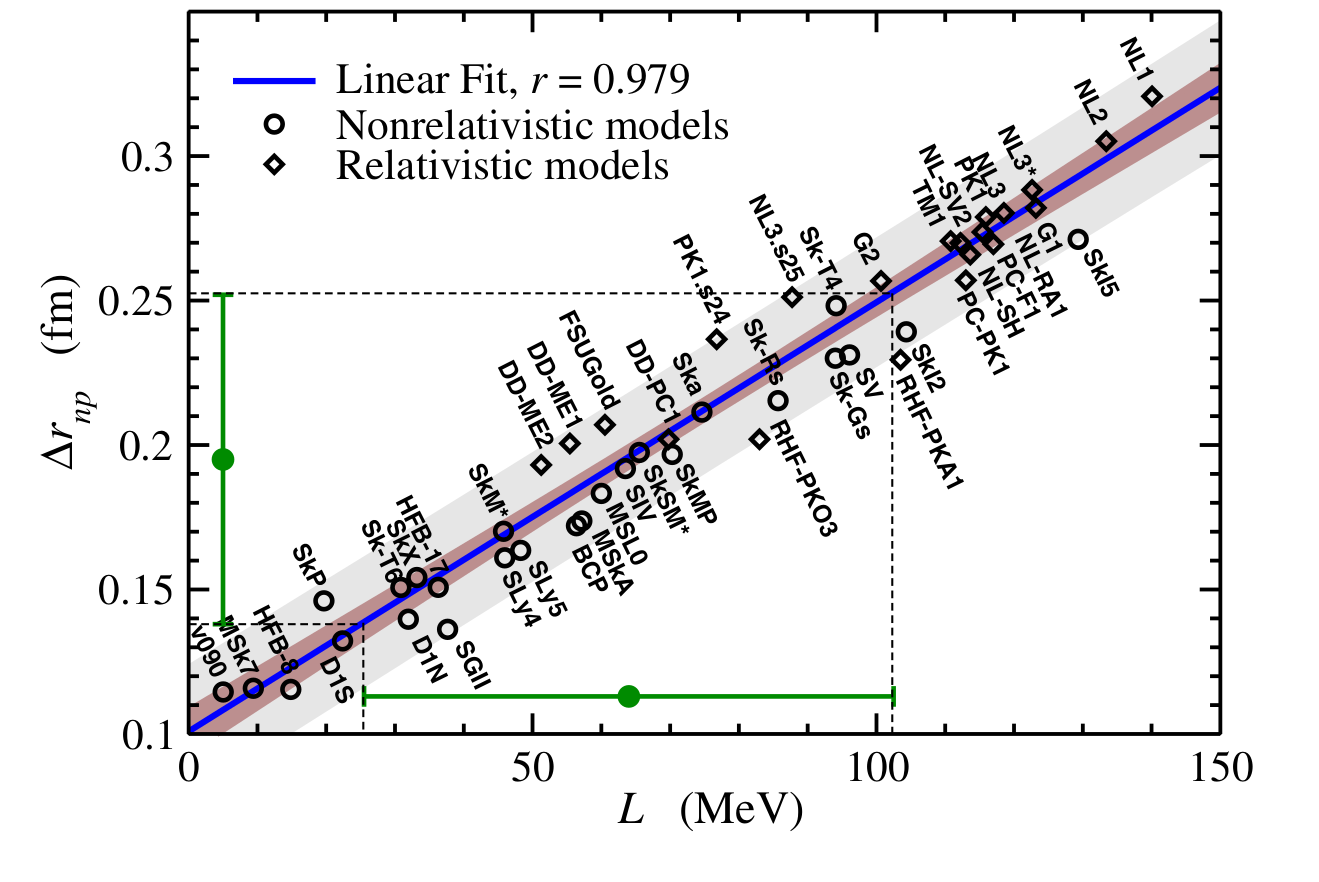
\includegraphics[width=0.5\linewidth]{R_skin_vs_L}
    \caption{Correlation between \Pb neutron skin thickness against slope of the
    symmetry energy ($L$). The linear fit is $\Delta r_{np} = 0.101 + 0.00147 L$.
    \cite{PhysRevLett.106.252501}}
\end{figure}

Being such an important parameter, great efforts have been devoted to extract $S$ 
and $L$. Comparing Eq.~\ref{eq:modified-mass-formula-2} and \ref{eq:symmetry-energy},
we can directly get:
\begin{equation}
    S(\rho) \approx -a_A
% S(\rho) = -a_A + \frac{L}{3}\frac{\rho - \rho_0}{\rho_0}
\end{equation}
The problem is this tells only the symmetry energy at the nuclear density ($\sim 1 \times 10^{44}\ \mathrm{m}^{-3}$).
It says nothing about the symmetry energy at other density values, especially at the nuclear
saturation density ($\sim 1.5 \times 10^{44}\ \mathrm{m}^{-3}$), let along the density
dependence of the symmetry energy. 

A more practical strategy to calculate $S(\rho)$ is the energy density functionals (EDF), 
which fits the binding energy throughout the nuclear mass table to find out the best EDF,
then use it to calculate $S(\rho)$. Fitting parameterizations are constrained
by nuclear density, point-proton RMS radii and nuclear binding energies. 
The issue is many EDFs can fit equally well with these constraints, but have quite 
different $L$ values, as shown in Fig.~\ref{fig:neutron_EOS}.
An experiment that could identify $S$ ($L$) value without model dependence, 
would be helpful in understanding the symmetry energy and the EOS.
\begin{figure}[!h]
    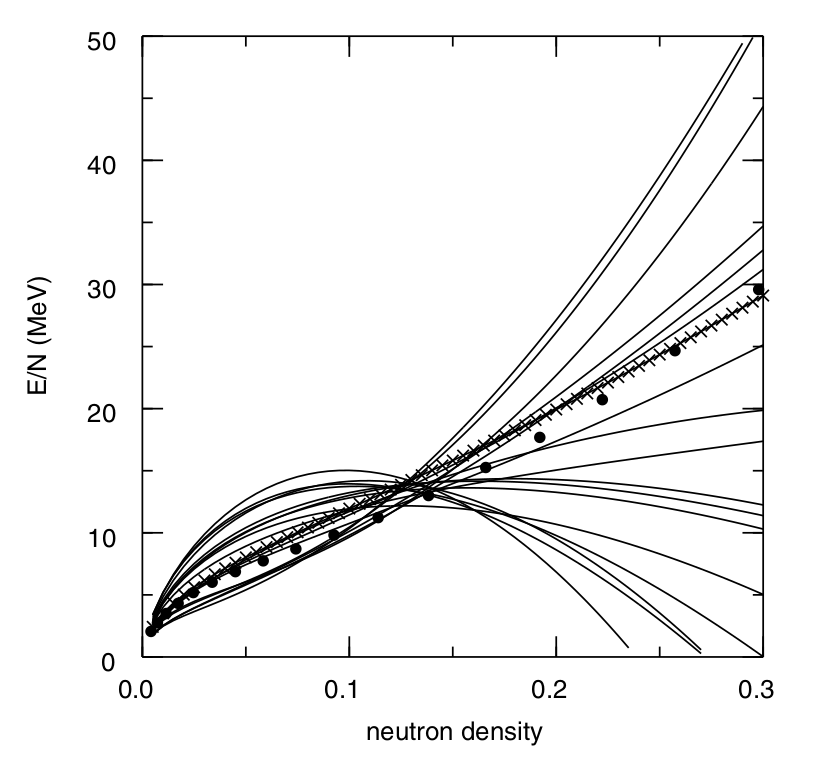
\includegraphics[width=0.48\linewidth]{S_vs_rho_n}
    \hfill
    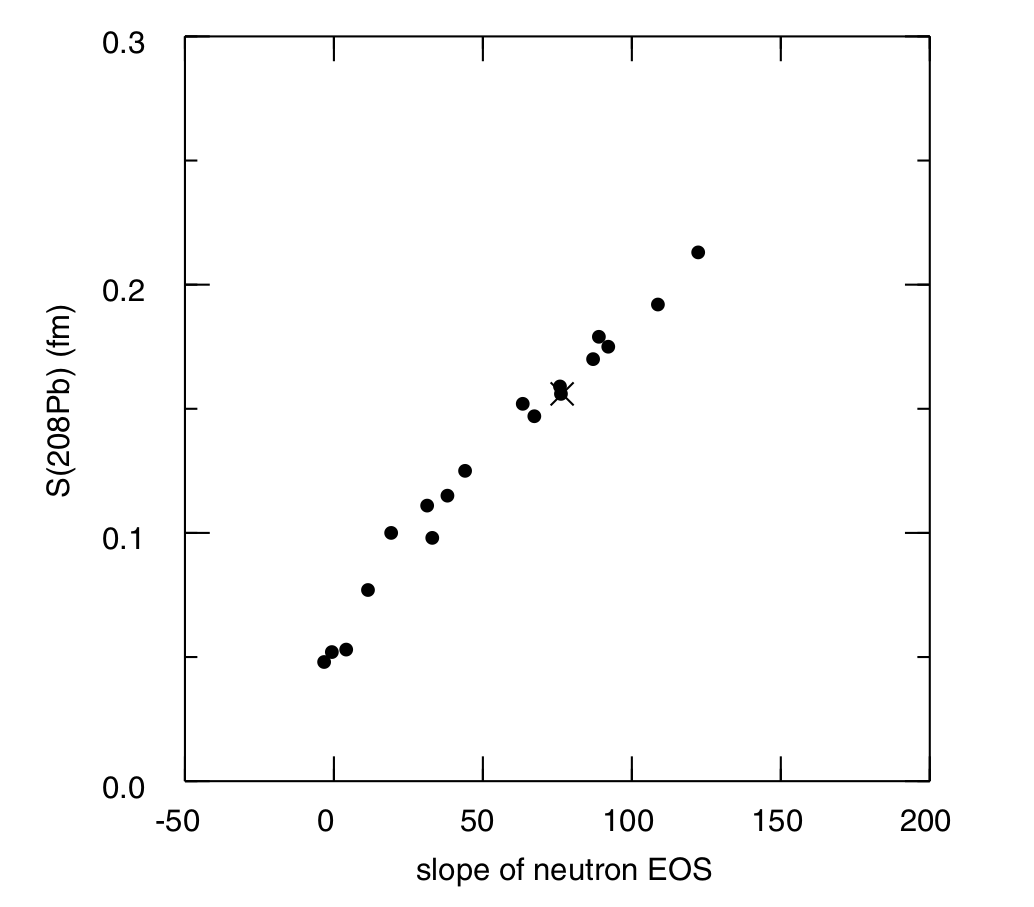
\includegraphics[width=0.49\linewidth]{S_Pb_in_S_N_EOS}
    \caption[Neutron EOS with different slope values]
    {Left: Neutron EOS for 18 Skyrme \cite{Skyrme} parameter sets. The filled circles are
    the Friedman-Panharipande (FG) variational calculations and the crosses are SkX predictions
    \cite{PhysRevC.58.220}.
    One can see that different models have very different symmetry energies.
    Right: Symmetry energy for nuclear EOS (in units of MeV $\mathrm{fm}^3$/neutron) 
    at $\rho_n = 0.1$~neutron/fm${}^3$ vs the S value in \Pb for 18 Skyrme parameter sets. 
    The cross is SkX. Determination of S in \Pb will greatly constrain the 
    possible candidates.
    \cite{PRL.85.5296}.
    }
    \label{fig:neutron_EOS}
\end{figure}
% experiments that measure L

% neutron skin
% The method to measure L in lab is to measure the neutron skin thickness of 
% neutron rich nuclei. For symmetric nuclei (N = Z), the protons and neutrons are
% expected to distribute uniformly. While for neutron-rich nuclei, the extra 
% neutrons are pushed out against the surface tension\cite{PRL.85.5296}, therefore
% forming a neutron skin. 
  
%%%%%%%%%%%%%%%%%%%%%%%%%%%%%%%%%%%%%%%%%%%%%%%%
\section{Nuclear Structure and Neutron Stars}
Unlike particle physics, there is no nuclear standard model that can describe
static properties and dynamics of atomic nuclei, such as the ground state binding energy,
nuclear size and excitation spectrum. 

The fundamental building blocks of nuclei are quarks and gluons. Theoretically, 
all properties of a nucleus can be derived directly from interactions
of these elementary particles using QCD. Many groups do work in this direction, 
trying to derive nuclear structure from the underlying QCD directly. 
Unfortunately, at the low energy scale where nuclei lie in, the non-perturbative nature of 
QCD makes the problem so complicated that even the state-of-the-art lattice QCD
technique can resolve only a small nuclear system with a few nucleons.
This suggests that quarks and gluons are not the best degrees of freedom to describe nuclei, 
up to now.

% first problem: nuclear forces governed by QCD, which is non-perturbative at low energy
Instead of quarks and gluons, nucleons and their intermediary particles pions,
being the direct components of nuclei, are a more natural choice of degrees of freedom for
the description of nuclei.
This was how physicists studied a nuclear system in the beginning (1930s \cite{10.1143/PTPS.1.1}). 
Many nuclear models were developed based on the meson-exchange phenomenology, called	% FIXME reference
phenomenological interactions. % up to the mid 1990s.
With the uncovering of QCD, this approach was re-discovered from the aspect of QCD:
quarks and gluons are confined in colorless nucleons and pions, the nuclear force
is just the residual interaction between quarks and gluons. Being rooted in the underlying
QCD, it is appropriate to describe nuclear systems in terms of nucleons and pions.

%%%%%%%%%%%%%%%%%%%%%%%%
\subsection{Ab-initio Method}
Though we don't know how nuclear force emerges from the underlying QCD interaction,
both the force and the interaction should share the same properties, 
especially the same symmetries and symmetry-breaking patterns. 
% among which, the most important one is the spontaneously broken chiral symmetry.
Based on this idea, in 1990s, S. Weinberg proposed a new framework: chiral 
effective field theory ($\chi$EFT), which is an effective realization of the 
underlying QCD Lagrangian based on chiral symmetry \cite{WEINBERG1979327}.

% All possible terms that are consistent with the underlying QCD symmetry.

Ab-initio methods try to calculate the wave function of nuclei by solving the
many-body Schr\"{o}dinger equation:
\begin{equation}
    H\ket{\psi} = E\ket{\psi}
\end{equation}
where the Hamiltonian is
\begin{equation}
    H = T + V = \frac{1}{A} \sum_{i<j}^A \frac{(\vec{p}_i - \vec{p}_j)^2}{2m} 
	+ \sum_{i<j}^A V_{ij}^{NN} + \sum_{i<j<k}^A V_{ijk}^{NNN} + \cdots
\end{equation}

$\chi$EFT requires that the potential should follow the same symmetries of QCD,
like spacetime translation, rotation, parity transformation, etc. Most importantly, $V$ should
preserve the spontaneously broken chiral symmetry. Constrained by these symmetries,
the operator for the potential takes the form of
\begin{equation}
    \mathds{O}_V = \{\mathds{1}, \vec{\sigma}_i \cdot \vec{\sigma}_j, \vec{L} \cdot \vec{S}, S_{ij}\} 
	\times \{\mathds{1}, \vec{\tau}_i \cdot \vec{\tau}_j\}
\end{equation}
where $\vec{\sigma}_i \cdot \vec{\sigma}_j$ ($\vec{\tau}_i \cdot \vec{\tau}_j$) 
denotes the spin (isospin) interaction, 
$\vec{L} \cdot \vec{S}$ indicates the spin-orbit interaction and tensor interaction
is represented by
\begin{equation}
    S_{ij}(\vec{x}) = 3(\vec{\sigma_i} \cdot \hat{\vec{x}})(\vec{\sigma}_j \cdot \hat{\vec{x}}) - \vec{\sigma}_i \cdot \vec{\sigma}_j
\end{equation}
where $\hat{\vec{x}}$ is the unit vector along vector $\vec{x}$.

The typical momentum (soft scale) in nuclei is $p \sim m_\pi \sim \mathds{O}(100\ \mathrm{MeV})$, 
while the short-range structure involving heavier meson (hard scale) is about 
$\Lambda_\chi \sim m_\rho \sim \mathds{O}(700 \ \mathrm{MeV})$. 
The clear gap between the soft and hard scales allows the separation of the 
long-range force from the short-range one, as shown in Fig.~\ref{fig:nuclear_potential}. 
The `effective' in the name of $\chi$EFT refers to the fact that only the 
long-range pion exchange in the low-energy scale will be considered, 
while heavier mesons will be integrated out as low-energy constants (LECs), 
which are phenomenologically fitted. 
\begin{figure}[!h]
    \centering
    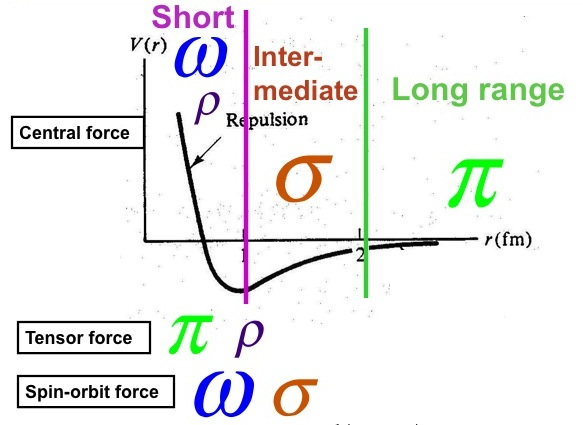
\includegraphics[width=0.5\linewidth]{nuclear_force}
    \caption{Separation of nuclear forces.}
    \label{fig:nuclear_potential}
\end{figure}

With the effective theory, one can expand the potential in terms of
$\left(\frac{Q}{\Lambda_\chi}\right)^\nu$, where Q is the momentum transfer
between two nucleons and $\Lambda_\chi$ is the cut off scale where short-range 
interactions becomes important, and
finally $\nu$ is the power, defining the order of interactions. As shown in
Fig.~\ref{fig:nuclear_interactions_in_order}.
\begin{equation}
    V = \sum_i V^{(i)} = V^{(0)}_{LO} + V^{(2)}_{NLO} + V^{(3)}_{NNLO} + V^{(4)}_{NNNLO} \cdots
\end{equation}
In this way, one can calculate nuclear force to any precision, by including
more higher order terms, if not limited by computing power.

\begin{figure}[!h]
    \centering
    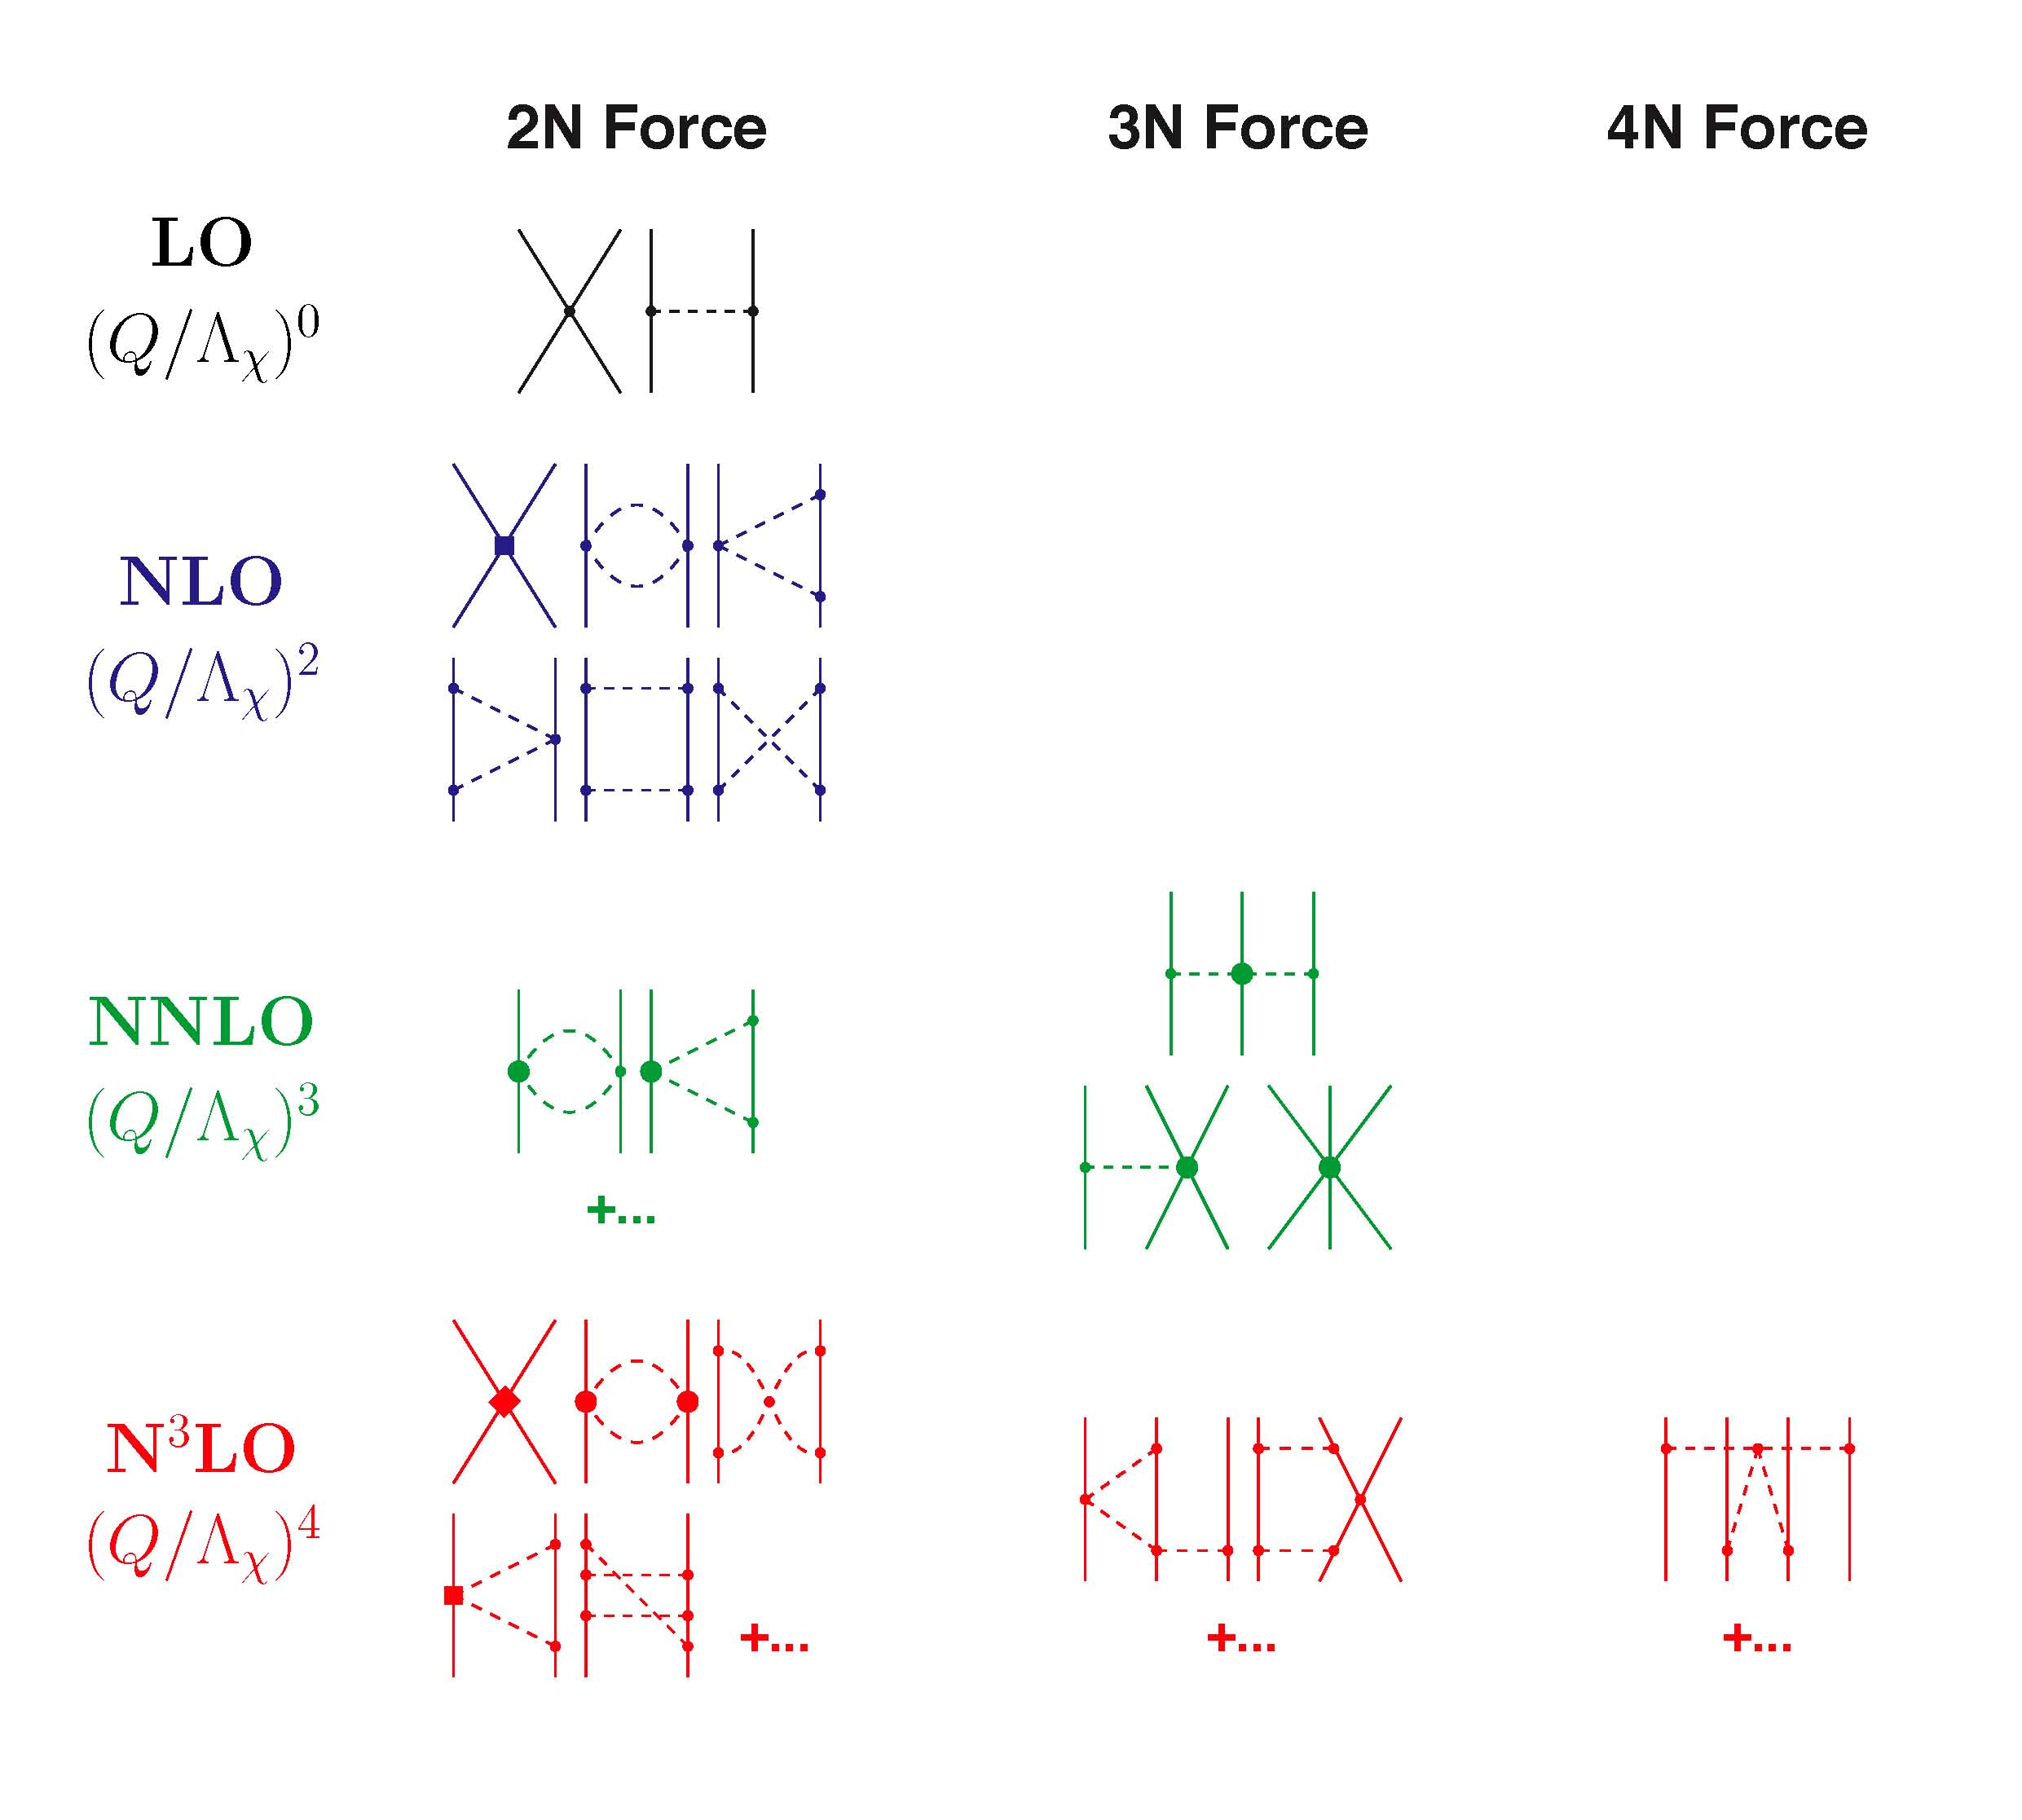
\includegraphics[width=0.5\linewidth]{nuclear_force_diagrams}
    \caption[Feynman diagrams for nuclear interactions]
    {Feynman diagrams for nuclear interactions. Solid lines refer to    
    nucleons while dashed lines represent exchanged pions. The first column     
    shows nucleon-nucleon force, and the following two columns correspond to three-nucleon
    and four-nucleon forces. Rows show diagrams of leading order (LO), next-to-leading order (NLO) and so forth.}
    \label{fig:nuclear_interactions_in_order}
\end{figure}

For example, the $1\pi$-exchange potential between two nucleons is:
\begin{equation}
    V_{2N}^{1\pi} = -\frac{g_A^2}{4F_\pi^2}
    \frac{(\vec{\sigma}_1\cdot\vec{q})(\vec{\sigma}_2\cdot\vec{q})}{\vec{q}^2 + M^2_\pi}
    \vec{\tau}_1\cdot\vec{\tau}_2 
\end{equation}
where $g_A$ and $F_\pi$ are the axial-vector coupling constant and the pion 
decay constant.

Once the nuclear force potential is selected, one can solve the Schr\"{o}dinger 
equation to get eigenstate wave-functions, from which various properties can be extracted. 
With the help of the many-body methods, like self-consistent Green's function,
coupled cluster and renormalization group, etc. ab-initio method can be extended
to nuclei of multiple nucleons.
% FIXME reference from each method

\begin{figure}[!h]
    \centering
    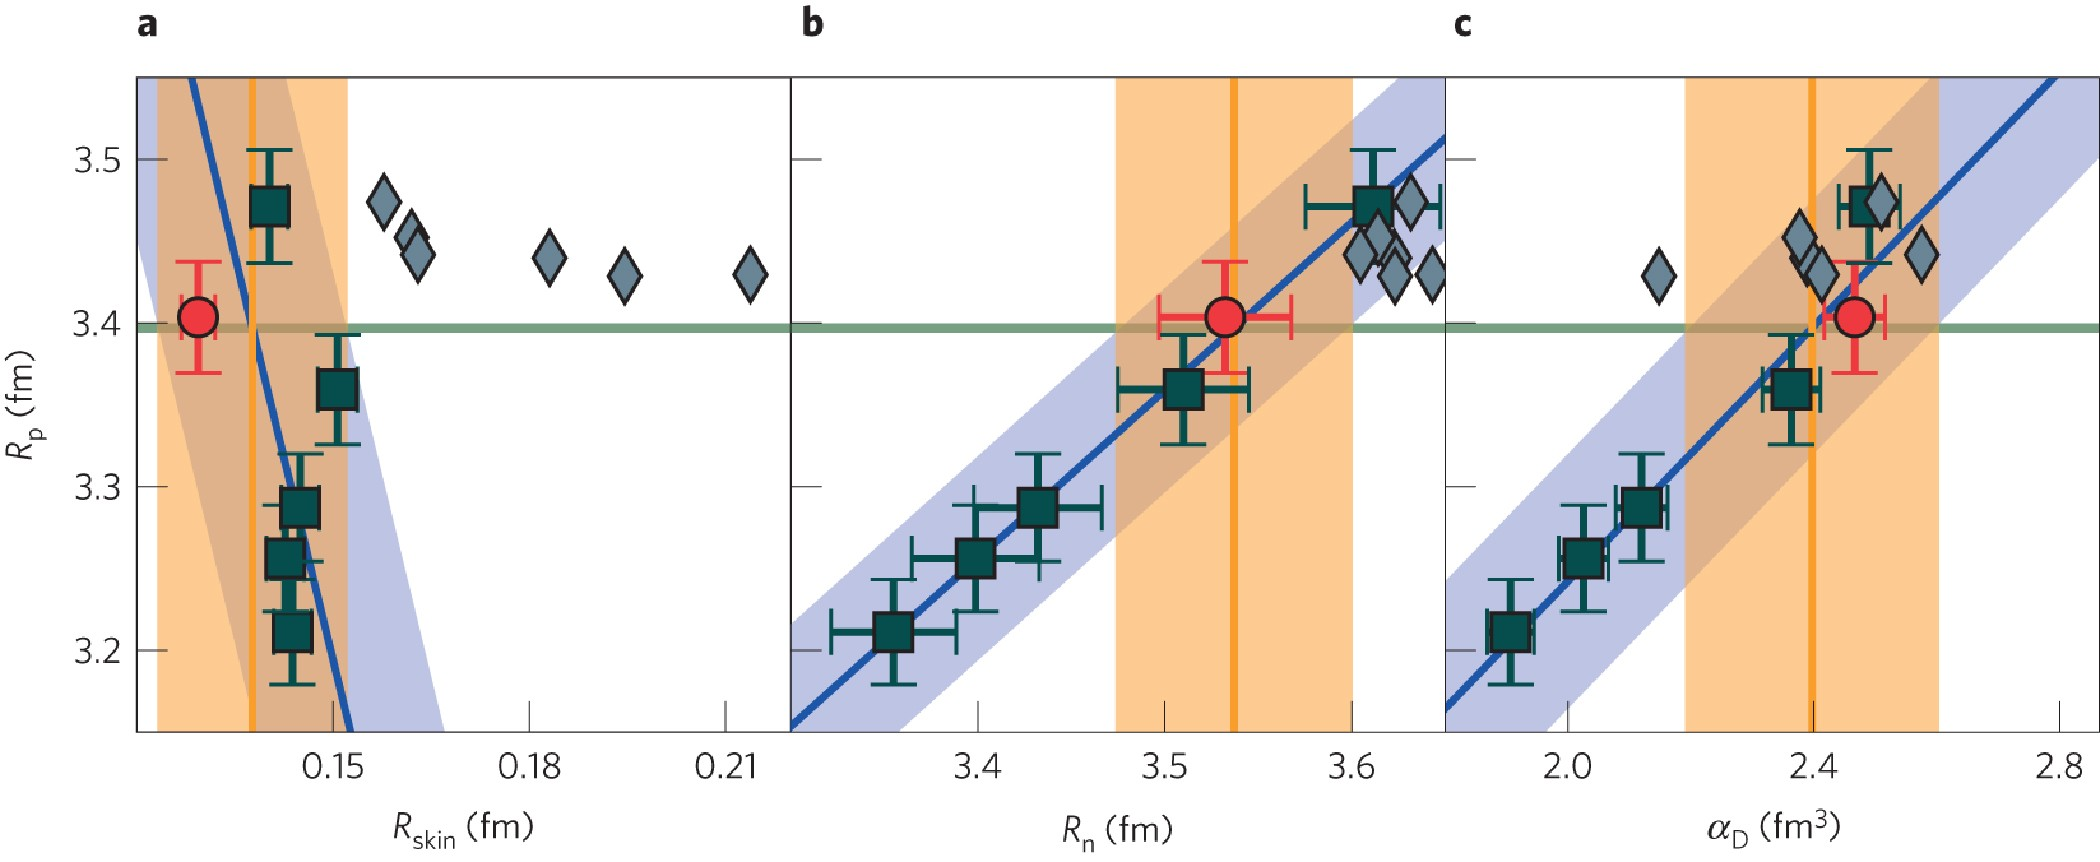
\includegraphics[width=0.8\linewidth]{ab_initio-Ca48_1}
    \caption[An ab-initio calculation of the neutron skin thickness of \Ca.]
    {An ab-initio calculation of the neutron skin thickness of \Ca.
    From left to right, neutron skin thickness (a), neutron radius (b) and
    electric dipole polarizability (c) of \Ca are plotted versus its proton 
    radius. The ab-initio predictions are shown as red circles and dark squares,
    while DFT results are represented by gray diamonds. The blue line represents 
    a linear fit to ab-initio predictions and the blue band is the corresponding
    uncertainty of the blue line. The horizontal green line marks the experimental
    value of $R_p$, whose intersection with the blue line and the blue band yields
    the vertical orange line and orange band, respectively. \cite{Hagen2016}.}
\end{figure}

\begin{comment}
Deviation of ab-initio result and observation for heavy nuclei indicates the 
importance of higher-order interactions.

\begin{equation}
    \CL_{eff} = \CL_{\pi\pi} + \CL_{\pi N} + \CL_{NN} + \cdots
\end{equation}

three-nucleon forces are hard to observe directly, they increase the pressure of
neutron matter and therefore the neutron skin thickness of both \Pb and \Ca.

three-nucleon force term
\begin{itemize}
    \item Long-range two-pion exchange
    \item Medium-range one-pion exchange
    \item Short range three-nucleon contact
\end{itemize}
\end{comment}
%%%%%%%%%%%%%%%%%%%%%%%%
\subsection{Nuclear Density Functional Theory (DFT)}
% The second problem is many-body problem
Despite the success of ab-initio methods with light and some medium nuclei, 
they are still unable to deal with heavy nuclei, because the required computing resources 
grow exponentially with the number of nucleons.
Instead of building the nuclear theory from the bottom up, one may do it the opposite
way, start from nuclear phenomenology, and try to go back to the underlying
QCD. The method developed in this way is nuclear DFT.

The DFT method originats from solid-state physics, where it was originally used to deal with
many-electron problem. It is based on the Hohenberg and Kohn (HK) theorem \cite{PhysRevC.57.3430}, 
which says one can write the total energy of a system
based on the fermion (electron) density (density functional), 
then minimization of this density functional leads to the ground state 
density distribution. In this way, one can greatly reduce the number of degrees of freedom, 
from 3N to 3. The only problem is that the HK theorem 
doesn't tell us how to construct such a density functional.

Nuclear interactions are more complicate than the Coulomb interaction, 
because three-nucleon interaction is not negligible. Fortunately, the nuclear interaction
is short-range. Given the experimental observation that the nucleon mean
free path in nuclei is about or larger than the nuclear radius, 
nucleons don't experience nuclear interaction frequently. This validates the use
of the mean-field method, namely nucleons move in a one-body potential which averages 
over interactions with all other nucleons. The most widely used one is the Woods-Saxon
potential.
% FIXME reference

Given the Hamiltonian of a nuclear system:
\begin{equation}
    H = \sum_i^N -\frac{\hbar^2}{2m}\nabla_i^2 + \frac{1}{2} \sum_{i\neq j=1}^N V(i, j)
\end{equation}
The Hartree-Fock (HF) energy of the sytem is:
\begin{equation}
    E_{HF}(\rho) = \bra{\Phi} H \ket{\Phi}
\end{equation}
where $\ket{\Phi}$ is the Slater determinant made up with the single-particle wave 
function $\ket{\phi}$.

The HK theorem states that:
\begin{equation}
    \frac{\delta}{\delta\rho(\vec{r})} \left( E_{HF} - \epsilon\int d^3r' \phi^*_j(\vec{r}')\phi_j(\vec{r}') \right) = 0
\end{equation}
With
\begin{equation}
    \rho(\vec{r}) = \sum_i^N \phi_i^*(\vec{r})\phi_i(\vec{r})
\end{equation}
It leads to the well-known HF equations:
\begin{equation}
    \begin{aligned}
	-\frac{\hbar^2}{2m}\nabla^2\phi_j(\vec{r}) 
	+ \sum_{l=1}^N \int d^3\vec{r}' \phi^*_l(\vec{r}') V(\vec{r}, \vec{r}') (\phi_l(\vec{r}')\phi_j(\vec{r}) - \phi_l(\vec{r}')\phi_l(\vec{r}'))
	&= \epsilon_j\phi_j(\vec{r})	\\
	\bra{j}\frac{-\hbar^2}{2m}\nabla^2\ket{j} + \sum_{l=1}^N \bra{jl}V(1-P_{12})\ket{jl} = \epsilon_j
    \end{aligned}
\end{equation}
where $P_{12}$ exchanges particles 1 and 2. So the total energy is:
\begin{equation}
    E_{HF} = T + \frac{1}{2}\sum_{jl} \int d^3r d^3r' \phi_j^*(\vec{r}')\phi_l^*(\vec{r}')V(\vec{r}, \vec{r}') (\phi_j(\vec{r}')\phi_l(\vec{r}') - \phi_l(\vec{r}')\phi_j(\vec{r}'))
\end{equation}
where T is the kinetic energy.

By knowing the interaction (potential term $V(\vec{r}, \vec{r}')$), 
one can calculate the density distribution and therefore the total 
energy of the system, and other properties. One successful model is the Skyrme force
\begin{equation}
    \begin{aligned}
	V_{\text{Skyrme}}(\vec{r}_1, \vec{r}_2) &= t_0 (1 + x_0 P_\sigma)\delta(\vec{r}_1 - \vec{r}_2) 
	+ \frac{1}{2}t_1 (1 + x_1 P_\sigma) \left( \vec{k}^{\dag2}\delta(\vec{r}_1 - \vec{r}_2) + \delta(\vec{r}_1 - \vec{r}_2)\vec{k}^2 \right)    \\
	&+ t_2(1 + x_2 P_\sigma)\vec{k}^\dag \cdot \delta(\vec{r}_1 
	    - \vec{r}_2)\vec{k} + \frac{1}{6} t_3 (1 + x_3 P_\sigma)\delta(\vec{r}_1 - \vec{r}_2) \rho^\alpha\left( \frac{\vec{r}_1 + \vec{r}_2}{2} \right) \\
	&+ iW_0 (\vec{\sigma}_1 + \vec{\sigma}_2) \cdot \vec{k}^\dag \times \delta(\vec{r}_1 - \vec{r}_2) \vec{k}
    \end{aligned}
\end{equation}
which has up to 10 parameters that are constrained by the experimental data, like
nuclear mass, radius and binding energy.

\bigskip
By measuring the neutron skin thicknesses of \Pb and \Ca, we can verify the
creditabilities of these ab-initio and DFT methods, and greatly constraint the
parameter space in each model, helping to develop a more general nuclear theory.

%%%%%%%%%%%%%%%%%%%%%%%%%%%%%%%%%%%%%%%%%%%%%%%%
\subsection{Neutron Stars}
% Take the neutron star \cite{Lattimer.2001} as an example. 
Neutron star is the densest celestial body known, the pressure due to gravity is so strong
that even atoms inside the star collapse, crushing together electrons
and protons into neutrons, hence the name of neutron star. Primarily neutron
stars are observed either as pulsars or in binary systems. By exploring basic properties of
neutron stars, we will touch some fundamental questions that are shared between nuclear physics 
and astrophysics. For example:
\begin{itemize}
    \item What is the high density phase of QCD?
    \item What is the structure of many compact and energetic celestial bodies?
	and what determines their EM, neutrino and gravitational radiations?
\end{itemize}

In spite of a 18 orders of magnitude difference in their sizes (fm vs km), 
the neutron star and the nuclear neutron skin share the same EOS. 
It is the pressure of neutron-rich matter that supports the neutron skin 
against its surface tension and a neutron star against its gravity. 
So the neutron skin thickness and the size of a neutron star are connected,
through the pressure of neutron-rich matter, more specifically, the
density dependence of the symmetry energy $L$.
The larger the neutron skin thickness, the larger the symmetry energy slope $L$,
the larger the pressure, and therefore the larger the radius of a neutron star, 
at the same mass. 

Quantitatively, a neutron star has mostly neutrons and only a few protons, 
so its isospin asymmetry $\beta \approx 1$. Eq.~\ref{eq:symmetry-energy} is 
simplified to:
\begin{equation}
    e(\rho) = e(\rho, 0) + S(\rho)
\end{equation}
Pressure is derived to be:
\begin{equation}
    P = \rho^2\frac{de}{d\rho} \simeq \rho^2 \frac{dS}{d\rho} \approx \frac{L\rho^2}{3\rho_0}  \\
\end{equation}
We see that the pressure of neutron-rich matter depends on $L$. 

For a cold neutron star, the correlation between its radius and its pressure is \cite{Lattimer.2001}:
\begin{equation}
    R \simeq C(\rho, M) P^{0.23-0.26} 
\end{equation}
where $C$ is a coefficient that depends on the density $\rho$ and the stellar mass M.

Once the $L$ value is fixed by an experimental measurement of the neutron skin 
thickness in \Pb, one can calculate the radius of a cold neutron star. 
% A neutron star is expected to have a solid crust over a liquid core. The phase transition
% from the high density core to the low density crust depends on the properties of the
% neutron-rich matter. Specifically, the density dependence of the symmetry energy $L$.
% A thicker neutron skin in \Pb indicates a large value of $L$, or rapid rise of
% the symmetry energy with density, which leads to a low transition density in a neutron
% star.



%%%%%%%%%%%%%%%%%%%%%%%%%%%%%%%%%%%%%%%%%%%%%%%%%%%%%%%%%%%%%%%%%%%%%%%%
\section{Physics Beyond the Standard Model (SM)} 
% leptoquark, Z', SUSY
PVES experiments are always a promising avenue for the search of physics beyond the SM in precision frontier,
because of the high precision they can achieve.
The Feynman diagrams from falvor-conserving PVES are shown in Fig.~\ref{fig:BSM}
\begin{figure}[!h]
    \centering
\feynmandiagram[small, vertical' = a to b]{
    i1 [particle = $e^-$] -- [fermion] a -- [fermion] o1 [particle = $e^-$],
    a -- [photon, edge label={Q}, edge label'=$\gamma$] b,
    i2 [particle = N] -- [fermion] b -- [fermion] o2 [particle = N],
    };
\feynmandiagram[small, vertical' = a to b]{
    i1 [particle = $e^-$] -- [fermion] a -- [fermion] o1 [particle = $e^-$],
    a -- [scalar, edge label={Q}, edge label'=Z] b,
    i2 [particle = N] -- [fermion] b -- [fermion] o2 [particle = N],
    };
\feynmandiagram[small, vertical' = a to b]{
    i1 [particle = $e^-$] -- [fermion] a -- [fermion] o1 [particle = $e^-$],
    a -- [scalar, edge label={Q}, edge label'=Z'] b,
    i2 [particle = N] -- [fermion] b -- [fermion] o2 [particle = N],
    };
    \caption{Feynman diagrams of elastic eA scattering.}
    \label{fig:BSM}
\end{figure}

Knowing that the EM interaction is much larger than the neutral weak current and
the possible new interaction, we can approximate:
\begin{equation}
    |\CA_\gamma + \CA_Z + \CA_{\text{new}}|^2 \approx A^2_\gamma\left[ 1 + 2\frac{\CA_Z}{\CA_\gamma}
    + 2\frac{\CA_{\text{new}}}{\CA_\gamma} \right]
\end{equation}
If the new interaction amplitude $\CA_{\text{new}}$ is comparable to $\CA_Z$ or our measurement 
of $\CA_Z$ is precise enough, we will be able to distinguish any possible deviation,
prompting on the existance of new physics.

Any PV interaction can be described in the SM as:
\begin{equation}
    \mathcal{L}_{PV}  = -\frac{G_F}{\sqrt{2}}\left[ 
	\bar{e}\gamma_\mu\gamma_5 e (C_{1u}\bar{u}\gamma^\mu u + C_{1d}\bar{d}\gamma^\mu d)
      + \bar{e}\gamma_\mu e (C_{2u}\bar{u}\gamma^\mu\gamma^5 u + C_{2d}\bar{d}\gamma^\mu \gamma^5d)
	\right]
% https://doi.org/10.1140/epja/i2006-09-011-8
\end{equation}
where $C_{iq}$ is the constant coefficient predicted by the SM:
\begin{equation}
    \begin{gathered}
	C_{1q} \equiv 2g_A^e g_V^q	\qquad C_{2q} \equiv 2g_V^e g_A^q   \\
	g_A = I_3   \qquad g_V = I_3 - 2Q\sin^2\theta_W
    \end{gathered}
\end{equation}
These coefficients or their combinations give favorable experimental observables:
\begin{equation}
    \begin{aligned}
	C_{1u} &= -\frac{1}{2} + \frac{4}{3}\sin^2\theta_W   \\
	C_{1d} &= \frac{1}{2} - \frac{2}{3}\sin^2\theta_W   \\
	C_{2u} &= -\frac{1}{2} + 2\sin^2\theta_W   \\
	C_{2d} &= \frac{1}{2} - 2\sin^2\theta_W   \\
    \end{aligned}
    \Longrightarrow
    \begin{aligned}
	\tilde{\alpha} &= -C_{1u} + C_{1d} = -(1-2\sin^2\theta_W)	\\
	\tilde{\beta} &= -C_{2u} + C_{2d} = -(1-4\sin^2\theta_W)	\\
	\tilde{\gamma} &= -C_{1u} - C_{1d} = \frac{2}{3}\sin^2\theta_W	\\
	\tilde{\delta} &= -C_{2u} - C_{2d} = 0	\\
    \end{aligned}
\end{equation}
where $\theta_W$ is the weak mixing angle.

Most PVES experiments measure the weak charge (the weak mixing angle) directly, like
E158 at SLAC and the upcoming MOLLER at JLab. Compared to these experiments, PREX/CREX
are less sensitive to new physics, because PREX/CREX measurements involve many 
weak charge sources inside a nucleus and their distribution. Though new physics
is not the main goal of the PREX/CREX collaboration, the possibility for new physics 
is not completely cut off.

%%%%%%%%%%%%%%%%%%%%%%%%%%%%%%%%%%%%%%%%%%%%%%%%
\section{Symmetry and Asymmetry}
Symmetry is a powerful framework in modern physics. For any physical system, 
by applying the proper symmetry requirements, one can derive (guess) 
the Lagrangian of the system, and therefore properties and Equation Of Motion (EOM)
of the system.

Common space-time symmetries can be separated into continuous symmetries 
and discrete ones. Continuous symmetries include translation, rotation and
boost, while discrete symmetries have space reflection (P) and time reversal (T).
Another important discrete symmetry is charge conjugation (C).

Playing such a key role, the violation of any symmetry is also important.
Currently, it is widely accepted that continuous
symmetries are conserved by all interactions while weak interaction violates
some discrete symmetries, namely C, P, and their combination CP. There are some
speculations that the strong interaction can violate the CP symmetry, but no
experimental observation reported yet.

%%%%%%%%%%%%%%%%%%%%%%%%%%%%%%%%%%%%%%%%%%%%%%%%
\subsection{Parity Symmetry}
Parity symmetry is a discrete symmetry which states that the physical laws in
the mirror (reflection) world should be the same as that in the real world. 
\begin{figure}[!h]
    \centering
    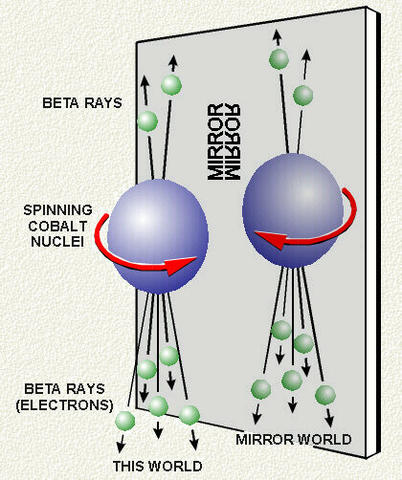
\includegraphics[width=0.4\linewidth]{parity}
    \caption{Schematic plot of space reflection.}
\end{figure}

The parity operation will flip the sign of any spatial coordinate:
\begin{equation}
    P: \vec{r} \rightarrow -\vec{r}
\end{equation}
The same for any spatial vector, like momentum ($\vec{p}$), angular momentum ($\vec{L}$)
and the EM vector potential ($\vec{A}$).

In the language of QM, the parity operator ($\hat{\pi}'$) will transform 
a wave function, as shown in Eq.~\ref{eq:parity_transformation}.
\begin{equation}
    \hat{\pi}'\psi(x, y, z) = \eta \psi(-x, -y, -z)
    \label{eq:parity_transformation}
\end{equation}
where $\eta$ is a coefficient picked up by the transformation. One would expect
the state goes back to itself after 2 times of parity transformations:
\begin{equation}
    |\hat{\pi}'^2 \psi(x, y, z)|^2 = |\psi(x, y, z)|^2
    \qquad
    \hat{\pi}'\psi(x, y, z) = e^{i\phi/2}\psi(-x, -y, -z)
\end{equation}
which means $\hat{\pi}'$ is an unitary operator. The pick up phase can
be absorbed into the operator to get the new parity operator (what we use hereafter): 
\begin{equation}
    \hat{\pi} = \hat{\pi}'e^{-i\phi/2}
\end{equation}
Then we have
\begin{equation}
    \hat{\pi}^2 = 1 
\end{equation}
So $\hat{\pi}$ has eigenvalues of $p = \pm 1$. States with eigenvalue of +1 are called
parity-even states and the others with eigenvalue of -1 the parity-odd states.

For any scalar potential, $V(\vec{r}) = V(r)$ ($[\hat{\pi}, V] = 0$), the parity 
operator $\hat{\pi}$ commutes with the Hamiltonian ($[\hat{\pi}, \CH] = 0$). 
So the energy eigenstates are also the eigenstate
of $\hat{\pi}$. Among these, the orbital angular momentum eigenstates are
of special interest. Given an orbital angular momentum $\vec{L}$ with z-axis projection
$L_z$, one will have:
\begin{equation}
    \hat{\pi}\ket{\vec{L}, L_z} = (-1)^L\ket{\vec{L}, L_z}
\end{equation}

Another quantity which is similar to the orbital angular momentum in most aspects but
different in parity is spin. Spin is also an angular momentum, but it is an 
intrinsic property, rather than a space-time motion. While $\hat{\pi}$ is an operation
of the space, spin is not affected by $\hat{\pi}$. So the parity of a spin state
is randomly assigned as long as particles and their anti-particles have opposite
parities: electron, proton and neutron are assigned even parity and
their anti-particles have odd parity.

Now we can discuss helicity, which is the projection of the spin on the momentum
direction: 
\begin{equation}
    H \equiv \frac{\vec{s}\cdot \vec{p}}{|\vec{s}\cdot\vec{p}|}
\end{equation}
If a particle's spin is parallel (anti-parallel) to its momentum, we call it a
right (left)-handed particle. Obviously, when we apply the parity operator to a helicity
eigenstate, we will flip its helicity because spin does not change and momentum 
will flip its sign, as shown in Fig.~\ref{fig:parity_eA_scattering_1}.
\begin{figure}[h!]
    \centering
    \begin{subfigure}[c]{0.44\linewidth}
	\begin{tikzpicture}[scale=0.8]
	    \begin{feynman}[transform shape]
		\vertex (i1) {$e^-$};
		\vertex [right=1.0cm of i1, inner sep=-2pt] (inspin) {\AxisRotator};
		\vertex [right=2.3cm of inspin] (ip);
		\vertex [right=2.8cm of ip] (i2) {A};
		\vertex [above right = 2cm and 2cm of ip] (o1) {$e^-$};
		\vertex [above right = 1cm and 1cm of ip] (outspin) {\AxisRotator[rotate=45]};
		\vertex [below left = 2cm and 2cm of ip] (o2) {A};

		\diagram* { {[edge=fermion]
		    (i1) --[edge label=$\vec{k}$] (ip) [dot] --[edge label = $\vec{k}'$] (o1),
		    (i2) --[edge label=$\vec{p}$](ip) [dot] -- [edge label = $\vec{p}'$]  (o2)},
		};
	    \end{feynman}
	\end{tikzpicture}
    \end{subfigure}
    $\overset{\hat{\pi}}{\Longrightarrow}$
    \hspace{0.2cm}
    \begin{subfigure}[c]{0.44\linewidth}
	\begin{tikzpicture}[scale=0.8]
	    \begin{feynman}[transform shape]
		\vertex (i1) {A};
		\vertex [right=2.8cm of i1] (ip);
		\vertex [right=2.3cm of ip, inner sep=-2pt] (inspin) {\AxisRotator};
		\vertex [right=1.0cm of inspin] (i2) {$e^-$};
		\vertex [above right = 2cm and 2cm of ip] (o1) {A};
		\vertex [below left = 1cm and 1cm of ip] (outspin) {\AxisRotator[rotate=45]};
		\vertex [below left = 2cm and 2cm of ip] (o2) {$e^-$};

		\diagram* { {[edge=fermion]
		    (i1) --[edge label=$\vec{p}$] (ip) [dot] --[edge label = $\vec{p}'$] (o1),
		    (i2) --[edge label=$\vec{k}$](ip) [dot] -- [edge label = $\vec{k}'$]  (o2)},
		};
	    \end{feynman}
	\end{tikzpicture}
    \end{subfigure}
    \caption{Parity transformation of the eA scattering}
    \label{fig:parity_eA_scattering_1}
\end{figure}

If parity is not conserved, there will be a difference between the two scattering 
processes in Fig.~\ref{fig:parity_eA_scattering_1}, which is exactly what we
measured in PREX-II/CREX. Experimentally, it is easier to flip the spin direction
rather than the momentum direction, as shown in Fig.~\ref{fig:parity_eA_scattering_2},
which is an equivalent plot of Fig.~\ref{fig:parity_eA_scattering_1}.
\begin{figure}[h!]
    \centering
    \begin{subfigure}[c]{0.48\linewidth}
	\begin{tikzpicture}[scale=0.8]
	    \begin{feynman}[transform shape]
		\vertex (i1) {$e^-$};
		\vertex [right=1.0cm of i1, inner sep=-2pt] (inspin) {\AxisRotator};
		\vertex [right=2.3cm of inspin] (ip);
		\vertex [right=2.8cm of ip] (i2) {A};
		\vertex [above right = 2cm and 2cm of ip] (o1) {$e^-$};
		\vertex [above right = 1cm and 1cm of ip] (outspin) {\AxisRotator[rotate=45]};
		\vertex [below left = 2cm and 2cm of ip] (o2) {A};

		\diagram* { {[edge=fermion]
		    (i1) --[edge label=$\vec{k}$] (ip) [dot] --[edge label = $\vec{k}'$] (o1),
		    (i2) --[edge label=$\vec{p}$](ip) [dot] -- [edge label = $\vec{p}'$]  (o2)},
		};
	    \end{feynman}
	\end{tikzpicture}
    \end{subfigure}
    \begin{subfigure}[c]{0.48\linewidth}
	\begin{tikzpicture}[scale=0.8]
	    \begin{feynman}[transform shape]
		\vertex (i1) {$e^-$};
		\vertex [right=1.0cm of i1, inner sep=-2pt] (inspin) {\AxisRotatorReversed};
		\vertex [right=2.3cm of inspin] (ip);
		\vertex [right=2.8cm of ip] (i2) {A};
		\vertex [above right = 2cm and 2cm of ip] (o1) {$e^-$};
		\vertex [above right = 1cm and 1cm of ip] (outspin) {\AxisRotatorReversed[rotate=45]};
		\vertex [below left = 2cm and 2cm of ip] (o2) {A};

		\diagram* { {[edge=fermion]
		    (i1) --[edge label=$\vec{k}$] (ip) [dot] --[edge label = $\vec{k}'$] (o1),
		    (i2) --[edge label=$\vec{p}$](ip) [dot] -- [edge label = $\vec{p}'$]  (o2)},
		};
	    \end{feynman}
	\end{tikzpicture}
    \end{subfigure}
    \caption{Equivalent plot of Fig.~\ref{fig:parity_eA_scattering_1}: flip spin 
    instead of momentum.}
    \label{fig:parity_eA_scattering_2}
\end{figure}
%%%%%%%%%%%%%%%%%%%%%%%%%%%%%%%%%%%%%%%%%%%%%%%%
\subsection{Parity Violation}
\begin{figure}[!h]
    \centering
    \begin{tikzpicture}[decoration={markings, 
	mark=at position 0.5 with {\arrow{stealth}}}
	]
	\begin{scope}
	    \coordinate (O) at (0, 0);
	    \filldraw[black] (O) circle (1pt);
	    \node[red, above] at (O) {$G_F$};
	    \draw[postaction={decorate}] (-2, 0) node[above] {n} -- +(2, 0);
	    \draw[postaction={decorate}] (O) -- +(2, 0)node[above] {$p$} ;
	    \draw[postaction={decorate}] (O) -- (35:2) node[above, sloped] {$e^-$};
	    \draw[postaction={decorate}] (O) -- (-35:2) node[above, sloped] {$\bar{\nu}_e$};
	\end{scope}

	\begin{scope}[xshift=5cm]
	    \coordinate (O) at (0, 0);
	    \filldraw[black] (O) circle (1pt);
	    \node[red, above] at (O) {$G_F$};
	    \draw[postaction={decorate}] (-2, 0) node[above] {n} -- +(2, 0);
	    \draw[postaction={decorate}] (O) -- +(2, 0)node[above] {$p$} ;
	    \draw[postaction={decorate}] (O) -- (35:2) node[above, sloped] {$e^-$};
	    \draw[postaction={decorate}] (-35:2) node[above, sloped] {$\nu_e$} -- (O);
	\end{scope}
    \end{tikzpicture}
    \caption{Fermi's interpretation of beta decay, current $j_{n \rightarrow p}$ 
    convert $n$ into $p$ and current $j_{\nu_e \rightarrow e}$ creates $(e, \ \bar{\nu}_e) $
    pair.}
\end{figure}
The story of parity violation traces back to the early age of particle physics. 
To explain the beta decay, Fermi proposed the four-fermion interaction 
(Fermi's interaction) in 1933 \cite{Fermi1934}, which is a low-energy limit of the 
weak interaction. In his theory, in analogy to the EM interaction (emission of a
photon by an electron: $\CM = ej_\mu^{em} A^\mu$) Fermi interpreted the $\beta$
decay as emission of the $(e, \bar{\nu}_e)$ pair, during the process a neutron converts
itself into a proton, therefore it is coupling of two currents:
\begin{equation}
    \CM = G_F (\bar{p} \mathds{O}^\mu n)(\bar{e} \mathds{O}_\mu \nu_e) 
	= G_F j^\mu_{(n\rightarrow p)} j_\mu^{(\nu_e\rightarrow e)}
\end{equation}
Where $G_F = 1.166 \times 10^{-5} \mathrm{GeV}^{-2}$ is the coupling constant that 
can be experimentally determined and $\mathds{O}$ represents 
the possible operators. Out of the five possible Lorentz invariant bi-linear forms 
(Scalar (S: $\mathds{O} = \mathds{1}$), pseudo-scalar (P: $\mathds{O} = \gamma^5$), 
Vector (V: $\mathds{O} = \mathds{\gamma^\mu}$), Axial vector (A: $\mathds{O} = \gamma^\mu\gamma^5$) 
and Tensor (T: $\mathds{O}=\sigma^{\mu\nu} = \frac{i}{2}(\gamma^\mu\gamma^\nu - \gamma^\nu\gamma^\mu)$)),
Fermi selected the vector current to keep in line with the EM interaction:
$j^\mu = \bar{u} \gamma^\mu u$.

%%%%%%%%%%%%%%%%%%%%%%%%
\subsubsection{V-A Theory}
In 1956, T. D. Lee and C. N. Yang, both being Fermi's students, postulated the
revolutionary idea of parity violation for solving the $\tau-\theta$ puzzle \cite{PhysRev.105.1671}, 
and they succeeded. Only one year later, their hypothesis was experimentally tested
by Wu et al in the decay of polarized ${}^{60}$Co nuclei \cite{PhysRev.105.1413}, 
establishing the fact that parity is not conserved in weak interactions and 
therefore the weak current is not a pure vector-like quantity. 
Based on the experimental result that parity is maximally violated (left-handed 
electrons interact weakly but right-handed don't) \cite{PhysRev.109.1015}, 
Sudarshan and Marshak \cite{PhysRev.109.1860.2}, also Feynman and Gell-Mann \cite{PhysRev.109.193},
updated Fermi's theory by replacing the vector current with a new current to 
accommodate parity violation:
\begin{equation}
    \CM = \frac{G_F}{\sqrt{2}}(\bar{p} \gamma^\mu(\mathds{1} - \gamma^5) n) (\bar{e} \gamma_\mu(\mathds{1} - \gamma^5) \nu_e)
\end{equation}
The factor of $\frac{1}{\sqrt{2}}$ was introduced to keep $G_F$ unchanged (Fermi's
original theory was not aware the fact that neutrino was left-handed only, resulting
in a decay phase space twice the real value in nature, to fix the problem, we can
either modify the value of $G_F$ or introduce a correction factor $\frac{1}{\sqrt{2}}$).
The V and A parts of the V-A theory refer to the vector and axial vector current, 
responsible for Fermi transitions and Gamow-Teller transitions respectively.
\begin{equation}
    j_V^\mu = \bar{u}\gamma^\mu u   \qquad 
    j_A^\mu = \bar{u}\gamma^\mu\gamma^5 u   
\end{equation}
The form of V-A as $\mathds{1} - \gamma^5$ happens to be the projection operator:
\begin{equation}
    P_R = \frac{\mathds{1} + \gamma^5}{2}   \qquad P_L = \frac{\mathds{1} - \gamma^5}{2}
\end{equation}
By definition of $\gamma$ matrix, one can easily verify that:
\begin{equation}
    \begin{gathered}
	\left(\frac{\mathds{1} - \gamma^5}{2} \right)^2 = \frac{\mathds{1} - \gamma^5}{2} 
	\qquad 
	\gamma^\mu \frac{\mathds{1} - \gamma^5}{2} = \frac{\mathds{1} + \gamma^5}{2} \gamma^\mu \\
	\gamma^\mu \frac{\mathds{1} - \gamma^5}{2} = \frac{\mathds{1} + \gamma^5}{2} \gamma^\mu \frac{\mathds{1}-\gamma^5}{2}
    \end{gathered}
\end{equation}
Then one can see the handedness of the new current:
\begin{equation}
    \CM = \frac{4G_F}{\sqrt{2}}(\bar{p} \gamma^\mu\frac{\mathds{1} - \gamma^5}{2} n) (\bar{e} \gamma_\mu\frac{\mathds{1} - \gamma^5}{2} \nu_e) 
    = \frac{4G_F}{\sqrt{2}}(\bar{p}_L \gamma^\mu n_L)(\bar{e}_L \gamma_\mu \nu_{e,L})
\end{equation}
Only left (right)-handed particles (antiparticles) can interact in the weak interaction.
In analogy to EM interaction, the coupling constant is proportional to a weak
charge (weak isospin $T_3$): right-handed fermions (left-handed antifermions) 
will have $T_3 = 0$ and left-handed fermions have the same weak charge. 

Given the fact that the charge current (which changes particle's electric charge) 
connects two types of fermions and lepton number is conserved in the weak interaction, 
it is natural to group them in a lepton doublet: 
\begin{equation}
    f_L = \begin{pmatrix} \nu_l \\ l \end{pmatrix}_L
\end{equation}
This implies that for left-handed fermions: $T=\frac{1}{2}, T_3 = \pm\frac{1}{2}$ 

Applying the V-A theory to more decay and scattering processes 
( $\mu^+ \rightarrow e^+ + \nu_e + \bar{\nu}_\mu$, $\pi^- \rightarrow l + \bar{\nu}_l$ etc.), 
we will have two charge currents:
\begin{equation}
    j_\mu^- = \bar{\nu}_{e, L} \gamma_\mu e_L	\qquad 
    j_\mu^+ = \bar{e}_L \gamma_\mu \nu_{e,L}
\end{equation}
which can be written in a more compact way w.r.t. the lepton doublet:
\begin{equation}
    j_\mu^\pm = \bar{f}_L \gamma_\mu t^\pm f_L
\end{equation}
where,
\begin{equation}
    t^+  =
    \begin{pmatrix}
	0   & 1	\\
	0   & 0	\\
    \end{pmatrix}
    = \frac{1}{2}(\sigma^1 + i\sigma^2)
    \quad
    t^-  =
    \begin{pmatrix}
	0   & 0	\\
	1   & 0	\\
    \end{pmatrix}
    = \frac{1}{2}(\sigma^1 - i\sigma^2)
\end{equation}
One can see clearly the SU(2) symmetry by the $t^\pm$ expression, the raising ($t^+$)
and lowing matrices ($t^-$) are the combination of the first two Pauli matrices.
Then one should consider the third component:
\begin{equation}
    j_\mu^3 = \bar{f}_L \gamma_\mu \frac{1}{2}t^3 f_L = \frac{1}{2} (\bar{\nu}_{e, L} \gamma_\mu \nu_{e, L} - \bar{e}_{L} \gamma_\mu e_L)
\end{equation}
This is a neutral current. The question is how to interpret it.
The only known neutral current at that time is the EM current, but this 
hypothetical term can't be the EM current because neutrino is neutral.
The neutral current remained a mystery until
Glashow, Salam and Weinberg postulated the GSW model, which interprets $j^3$ as
part of a more complete neutral current that includes $j^{em}$ -- the so-called
$SU(2)_L \times U(1)$.

%%%%%%%%%%%%%%%%%%%%%%%%
\subsubsection{W Bosons}
One problem with Fermi's theory is that the cross section ($\sigma \sim G_F^2 E^2$) 
will diverge at high energy, to which the solution was the introduction of
mediating mesons: $W^\pm$. Unlike photon that mediates EM interaction, W boson
is charged, and has a heavy mass implied from the short-range nature of the
weak interaction. The introduction of W fields just makes the weak interaction
more similar to the EM interaction:
\begin{equation}
    \CL = g_W(J^+W^+ + J^-W^-)
\end{equation}
\begin{figure}[!ht]
    \centering
    \begin{tikzpicture}[decoration={markings, 
	mark=at position 0.5 with {\arrow{stealth}}}
	]
	\begin{scope}
	    \coordinate (O) at (0, 0);
	    \filldraw[black] (O) circle (1pt);
	    \node[red, above left] at (O) {$\frac{G_F}{\sqrt{2}}$};
	    \draw[postaction={decorate}] (-2, 0) node[above] {n} -- +(2, 0);
	    \draw[postaction={decorate}] (O) -- +(2, 0)node[above] {$p$} ;
	    \draw[postaction={decorate}] (O) -- (35:2) node[above, sloped] {$e^-$};
	    \draw[postaction={decorate}] (-35:2) node[above, sloped] {$\nu_e$} -- (O);
	\end{scope}

	\begin{scope}[xshift=5cm]
	    \coordinate (O) at (0, 0);
	    \coordinate (P) at (-35:2);
	    \filldraw[black] (O) circle (1pt);
	    \filldraw[black] (P) circle (1pt);
	    \node[red, above] at (O) {$V_{ud}g_W$};
	    \draw[postaction={decorate}] (-2, 0) node[above] {n} -- +(2, 0);
	    \draw[postaction={decorate}] (O) -- +(2, 0)node[above] {$p$} ;
	    \draw[decorate, decoration=snake] (O) -- node[red, midway, below left] {$\frac{1}{M^2_W}$} (P);
	    \draw[postaction={decorate}] (P) -- +(20:1) node[above, sloped] {$e^-$};
	    \draw[postaction={decorate}] ($(P) + (-20:1)$) node[below, sloped] {$\nu_e$} -- (P);
	    \node[red, below] at (P) {$g_W$};
	\end{scope}
    \end{tikzpicture}
    \caption{W-boson exchange picture of $\beta$ decay}
\end{figure}

Given the similarity between weak interaction and EM interaction, it is natural
to unify them into a multiplet of gauge fields. Based on Yang and Mills' non-abelian 
gauge theory, Salam and Weinberg successfully came up with a unified 
framework for both interactions -- the SU(2)${}_\mathrm{L} \times$ U(1) structure first suggested 
by Glashow. The SU(2) part is generated by `weak isospin', the subscript L referring
to the fact that only left-handed fermions couple to gauge boson of SU(2), and the U(1)
part comes from the `weak hypercharge'. There are 4 vector bosons:
$$ W^1, W^2, W^3, B $$
These bosons will couple to both left-handed and right-handed fermions. For simplicity,
consider only the first generation leptons here:
\begin{equation}
    \psi_1 = \begin{pmatrix} \nu_e \\ e^-  \end{pmatrix}	\quad
    \psi_2 = \nu_{e,R}	\quad
    \psi_3 = e^-_R    \quad
\end{equation}

The left-handed doublet $\psi_1$ interacts with all bosons, 
so the covariant derivative is:
\begin{equation}
    D_\mu = \partial_\mu - ig\frac{\sigma^a}{2}W_\mu^a - ig'y_1B_\mu
\end{equation}
where $y_1$ is the hypercharge of $\psi_1$.
The corresponding coupling Lagrangian is:
\begin{equation}
    \CL_{int, L} = -i\bar{\psi}_1 \gamma^\mu (g\frac{\sigma^a}{2}W^a_\mu + g'y_1B_\mu) \psi_1
	= -i(g\vec{j}^\mu\vec{W}_\mu + g'y_1\bar{\psi}_1\gamma^\mu\psi_1 B_\mu)
\end{equation}
Right-handed singlets don't couple to weak vector bosons, 
therefore the covariant derivative for right-handed fermions is:
\begin{equation}
    D_\mu = \partial_\mu - ig'y_{2(3)}B_\mu
\end{equation}
$y_{2(3)}$ is the hypercharge of $\psi_{2(3)}$
and the Lagrangian:
\begin{equation}
    \CL_{int, R} = -ig'(y_2\bar{\psi}_2 \gamma^\mu \psi_2 + y_3\bar{\psi}_3\gamma^\mu \psi_3) B_\mu
\end{equation}
So the complete interacting Lagrangian is:
\begin{equation}
    \CL_{int} = \CL_{int, L} + \CL_{int, R} = -i(g\vec{j}^\mu \vec{W}_\mu + g'j^\mu_{Y} B_\mu)
    \label{eq:GSW}
\end{equation}
where $\vec{j}^\mu$ is the weak isospin current. It couples to a weak 
isotriplet of vector bosons: $\vec{W} = (W^1, W^2, W^3)$ with
coupling strength $g$; and the weak hypercharge current 
$j^\mu_{Y} = \sum_{i=1}^3 y_i\bar{\psi}_i\gamma^\mu\psi_i$ couples to 
an isosinglet vector boson $B^\mu$ with strength $g'$. 

%%%%%%%%%%%%%%%%%%%%%%%%
\subsubsection{Weak Neutral Current}
Because the GSW model preserves the SU(2) structure, 
it is obvious to reproduce the charged current:
\begin{equation}
    W^\pm = \frac{1}{\sqrt{2}}(W^1 \mp iW^2)	\quad
    j^\pm = j^1 \pm ij^2
\end{equation}
\begin{equation}
    j^1W^1 + j^2W^2 = \frac{1}{\sqrt{2}}(j^+W^+ + j^-W^-)
\end{equation}

As for the other 2 bosons, there is no way to satisfy $y_1 = y_2 = y_3$ and 
$g'y_i = eQ_i$ at the same time, so $B$ is not pure $A$ (photon). 
Since both fields are neutral, one needs to mix them to
get something matching experimental results:
\begin{equation}
    \begin{pmatrix}
	A   \\
	Z   \\
    \end{pmatrix}
    =
    \begin{pmatrix}
	\cos\theta_W	& \sin\theta_W	\\
	-\sin\theta_W	& \cos\theta_W	\\
    \end{pmatrix}
    \begin{pmatrix}
	B   \\
	W^3 \\
    \end{pmatrix} 
    \Leftrightarrow
    \begin{pmatrix}
	B   \\
	W^3 \\
    \end{pmatrix}
    =
    \begin{pmatrix}
	\cos\theta_W	& -\sin\theta_W	\\
	\sin\theta_W	& \cos\theta_W	\\
    \end{pmatrix}
    \begin{pmatrix}
	A   \\
	Z	\\
    \end{pmatrix} \\
\end{equation}
The mixing angle is known as the Weinberg angle. 

Rewrite Eq.~\ref{eq:GSW} in terms of $W^\pm$, $Z$ and $A$:
\begin{equation}
    \begin{aligned}
	i\CL = &\frac{g}{\sqrt{2}}(j^+W^+ + j^-W^-)	\\
	    &+ \sum_{i=1}^3\bar{\psi}_i\gamma^\mu \left\{ 
		\left[g\frac{\sigma^3}{2}\sin\theta_W + g'y_i\cos\theta_W\right] A_\mu
		+ \left[ g\frac{\sigma^3}{2}\cos\theta_W - g'y_i\sin\theta_W \right] Z_\mu 
	    \right\} \psi_i
    \end{aligned}
\end{equation}
where $g_W = g/\sqrt{2}$ is the coupling constant of weak charged current.

The neutral part can be expressed with corresponding charge:
\begin{equation}
    \begin{aligned}
	i\CL_{NC} &= \sum_{i=1}^{3} \bar{\psi}_i\gamma^\mu\psi_i
	\left[ 
	    \left(g\sin\theta_W I_3 + g'\cos\theta_W Y \right) A_\mu 
	    + \left(g\cos\theta_W I_3 - g'\sin\theta_W Y \right) Z_\mu 
	\right]	\\
	&= ej^\mu_{EM}QA_\mu + g_Zj^\mu_Z Q_Z Z_\mu \\
    \end{aligned}
\end{equation}
where $I_3$ is the weak isospin and $Y$ is the weak hypercharge. Similarly, $Q$ is
the EM charge in units of electron charge and $Q_Z$ is the weak neutral charge.
$e$ and $g_Z$ are coupling constant for EM and neutral weak interaction respectively.
With $I_3$ and $Y$ varying for different fermions, we have the following relationship:
% \begin{equation}
%     \begin{aligned}
% 	ej^{EM} &= g\sin\theta_Wj^3 + g'\cos\theta_Wj^Y	\\	
% 	g_Zj^{Z} &= g\cos\theta_W j^3 - g'\sin\theta_W j^Y	\\
%     \end{aligned}
% \end{equation}
\begin{equation}
    e = g\sin\theta_W = g'\cos\theta_W = \frac{gg'}{g^2 + g'^2}
\end{equation}
So the Weinberg angle is identified as:
\begin{equation}
    \tan\theta_W = \frac{g'}{g}
\end{equation}
and: 
\begin{equation}
    Q = I_3 + Y	\Longrightarrow Y = Q - I_3
    \label{eq:weak_hypercharge}
\end{equation}
The value of weak hypercharge depends on the definition, if one keeps the $\frac{1}{2}$
factor in the B current, then one will get:
\begin{equation}
    \frac{Y}{2} = Q - I_3   \Rightarrow Y = 2(Q-I_3)
\end{equation}
This is the traditional formula.
In this thesis we will use the definition of Eq.~\ref{eq:weak_hypercharge}.

As for the neutral weak current, the value of $g_Z$, $Q_Z$ and $J_Z$ depend on our choice, 
as long as:
\begin{equation}
    g_Z Q_Z J_Z = (g\cos\theta_W I_3 - g'\sin\theta_W Y)\bar{\psi}\gamma^\mu\psi 
\end{equation}
% To keep the uniformality of weak interaction at low energy limit, we can require:
% \begin{equation}
%     \frac{4G_F}{\sqrt{2}} = \frac{g_Z^2}{2M_Z^2} = \frac{g_W^2}{M_W^2}
% \end{equation}
% The factor of $1/2$ in Z coupling comes from the fact that Z can interact with both chiralities of fermions.
The traditional choice is:
\begin{equation}
    \begin{aligned}
	g_Z &= \frac{g}{\cos\theta_W} = \frac{e}{\sin\theta_W\cos\theta_W}  \\
	Q_Z &= I_e\cos^2\theta_W - Y\sin^2\theta_W = I_3 - Q\sin^2\theta_W  \\
    \end{aligned}
\end{equation}
One can also absorb $Q_Z$ into $J_Z$ to get:
\begin{equation}
    J_Z = \sum \bar{\psi}_i\gamma^\mu (I_3 - Q\sin^2\theta_W)\psi_i
	= \sum_f \bar{f}\gamma^\mu\frac{c_v - c_a\gamma^5}{2} f \\
\end{equation}
with 
\begin{equation}
    c_v = I_3 - 2Q\sin^2\theta_W    \quad c_a = I_3
\end{equation}
So we come to a striking prediction of the GSW model: the existance of the neutral weak interaction.
That was experimentally verified in 1973 in the Gargemlle neutrino experiment \cite{HASERT19741}.

%%%%%%%%%%%%%%%%%%%%%%%%
\subsubsection{PREX-II and CREX Observations}
What will be measured in PREX-II and CREX originates from the
interference of this neutral weak current and the EM current.

\begin{figure}[!h]
    \centering
\feynmandiagram[small, vertical' = a to b]{
    i1 [particle = $e^-$] -- [fermion] a -- [fermion] o1 [particle = $e^-$],
    a -- [photon, edge label={Q}, edge label'=$\gamma$] b,
    i2 [particle = N] -- [fermion] b -- [fermion] o2 [particle = N],
    };
\feynmandiagram[small, vertical' = a to b]{
    i1 [particle = $e^-$] -- [fermion] a -- [fermion] o1 [particle = $e^-$],
    a -- [scalar, edge label={Q}, edge label'=Z] b,
    i2 [particle = N] -- [fermion] b -- [fermion] o2 [particle = N],
    };
    \caption{Feynman diagrams of elastic e-N scattering in PREX-II/CREX.}
\end{figure}

\begin{equation}
    \CA_{PV} = \frac{\left( \frac{d\sigma}{d\Omega} \right)^R - \left( \frac{d\sigma}{d\Omega} \right)^L}
    {\left( \frac{d\sigma}{d\Omega} \right)^R + \left( \frac{d\sigma}{d\Omega} \right)^L}
    = \frac{|\CM^R|^2 - |\CM^L|^2}{|\CM^R|^2 + |\CM^L|^2}
\end{equation}
where: $\CM^{R, L} = \CM_{\gamma} + \CM_Z^{R,L}$. Because EM amplitude is much 
larger than the weak amplitude: $\CM_\gamma >> \CM_Z^{R, L}$

\begin{equation}
    \begin{aligned}
	\CA_{PV} &\approx \frac{2\CM_\gamma (\CM_Z^R - \CM_Z^L)}{2\CM^2_\gamma}	\\
	    &= \frac{\CM_Z^R - \CM_Z^L}{\CM_\gamma} \propto \frac{\left( \frac{d\sigma}{d\Omega} \right)_{\text{W}}}{\left( \frac{d\sigma}{d\Omega} \right)_{\text{EM}}}	\\
	    &= \left(\frac{\CM_Z^R - \CM_Z^L}{\CM_\gamma}\right)_{point} \times \frac{Q_{W}}{Z}\frac{F_{W}(Q^2)}{F_{EM}(Q^2)}    \\
	    &\approx \frac{g^2_Z/M_Z^2}{e^2/Q^2} \frac{(j_Z^{e,R} - j_Z^{e,L}) j_Z^n}{j_\gamma^e j_\gamma^p}
		\times \frac{Q_{W}}{Z}\frac{F_{W}(Q^2)}{F_{EM}(Q^2)} 	\quad (Q^2 << M_Z^2) \\
	    &= -\frac{8G_F/\sqrt{2}}{4\pi\alpha/Q^2} 
		\frac{(\bar{e}_L\gamma^\mu I_3e_L) \frac{1}{2}(\bar{n}_L \gamma_\mu I_3 n_L)}{(\bar{e}_L\gamma^\mu e_L)(\bar{p}\gamma_\mu p)}
		\times \frac{Q_{W}}{Z}\frac{F_{W}(Q^2)}{F_{EM}(Q^2)}    \\
	    &= -\frac{G_F Q^2}{4\pi\alpha\sqrt{2}} \frac{Q_{W}}{Z}\frac{F_{W}(Q^2)}{F_{EM}(Q^2)}
    \end{aligned}
    \label{eq:asymmetry}
\end{equation}
The weak isospin for electron and neutron is: $I_3(e^-) = I_3(n) = -\frac{1}{2}$.
The factor of $\frac{1}{2}$ in line 5 of Eq.~\ref{eq:asymmetry} arises from
the fact that the target is unpolarized. In the low $Q^2$ region of $Q^2 \sim 0.01 - 1 \mathrm{GeV} ^2$,
one can estimate the PV asymmetry as 
\begin{equation}
    -\CA_{PV} \sim \frac{G_F Q^2}{4\pi\alpha \sqrt{2}} \lesssim 10^{-7} - 10^{-4}
\end{equation}

The FFs can be further decomposed into point-nucleon FFs:
\begin{equation}
    \begin{aligned}
	F_{EM}(q) &= Q^\gamma_p F_p(q) + Q^\gamma_n F_n(q)  = F_p(q)	\\
	F_{W}(q)  &= Q^Z_p F_p(q) + Q^Z_n F_n(q)  \\
    \end{aligned}
\end{equation}
Where $Q^\gamma$ and $Q^Z$ are the EM charge and weak charge respectively.
$F_p(q)$ and $F_n(q)$ are the FFs of point-proton and neutron density distributions. 
\begin{equation}
    F_{p,n}(q) = \int d^3r j_0(qr) \rho_{p,n}(r)
\end{equation}
For weak charges including radiative corrections
\begin{equation}
    \begin{gathered}
	Q^\gamma_p = 1  \qquad Q^\gamma_n = 0   \\
	Q^Z_p = 0.0719    \qquad Q^Z_n = -0.9877
    \end{gathered}
\end{equation}
Ignoring the proton's weak charge, one will get:
\begin{equation}
    \CA_{PV} = -\frac{G_FQ^2}{4\pi\alpha\sqrt{2}}\frac{Q_{wk}}{Z} \frac{F_n(q)}{F_p(q)} 
\end{equation}
A more precise result by including the proton's weak charge is:
\begin{equation}
    \CA_{PV} = -\frac{G_FQ^2}{4\pi\alpha\sqrt{2}}\frac{Q_{wk}}{Z}\left[ \frac{F_n(q)}{F_p(q)} - \frac{Z}{N}(1-4\sin^2\theta_W) \right]
    \label{eq:Apv}
\end{equation}

When ignoring the nuclear innner structure (at tree level), Eq.~\ref{eq:Apv} reduces to:
\begin{equation}
    \CA_{PV} = -\frac{G_F Q^2}{\pi\alpha\sqrt{2}} \left(\sin^2\theta_W + \frac{1}{4}\left[ \frac{N}{Z} - 1 \right] \right)
\end{equation}

%%%%%%%%%%%%%%%%%%%%%%%%%%%%%%%%%%%%%%%%%%%%%%%%%%%%%%%%%%%%%%%%%%%%%%%%
\section{Dynamics}
\begin{center}
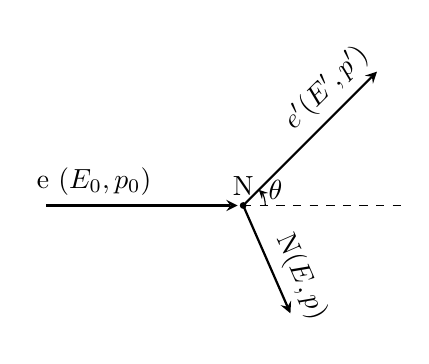
\begin{tikzpicture}
    \coordinate (N) at (0, 0);
    \coordinate (ein) at (-2.5, 0);
    \coordinate (eout) at (1.7, 1.7);
    \coordinate (p) at (0.6, -1.37);

    \filldraw[black] (N) circle (1pt);
    \node [above] at (N) {N};
    \draw[-stealth, thick] (ein) -- node [near start, above] {e ($E_0, p_0$)} ([xshift=-2pt]N);
    \draw[dashed] (N.east) -- +(2, 0);
    \draw[-stealth, thick] (N) -- node[near end, above, sloped] {$e' (E', p')$} (eout);
    \draw[-stealth, thick] (N) -- node[near end, above, sloped] {N($E, p$)} (p);
    \draw [-stealth] ([xshift=8pt]N) arc (0:45:8pt) node[right] {$\theta$};
\end{tikzpicture}
\end{center}

Energy and momentum are conserved in elastic scattering:
$$ E_0 + M = E' + E \qquad \vec{p}_0 = \vec{p}' + \vec{p} $$
where $M$ is the mass of the target nucleus.

Ignore the electron's mass, we have $E_0 \approx p_0$ and $E' \approx p'$:
\begin{equation}
    \begin{aligned}
	E^2 &= M^2 + \vec{p}^2 = M^2 + (\vec{p}_0 - \vec{p}')^2  \\
	    &= M^2 + (E_0 - E'\cos\theta)^2 + (E'\sin\theta)^2	\\
	    &= M^2 + E_0^2 + E'^2 - 2E_0E'\cos\theta	\\
	    &= (E_0 + M - E')^2
    \end{aligned}
\end{equation}

So we get:
\begin{equation}
    M(E_0 - E') = E_0E'(1-\cos\theta)   \Longrightarrow
    E' = \frac{ME_0}{M + E_0(1-\cos\theta)}
\label{eq:scattered_energy}
\end{equation}

$Q^2$ dependence on the scattering angle $\theta$ is calculated as:
\begin{equation}
    Q^2 = -q^2 = -[(E_0 - E')^2 - (\vec{p}_0 - \vec{p}')^2] = 2E_0E'(1-\cos\theta)
    \label{eq:Q2}
\end{equation}

%%%%%%%%%%%%%%%%%%%%%%%%%%%%%%%%%%%%%%%%%%%%%%%%%%%%%%%%%%%%%%%%%%%%%%%%
\section{Why Pb208 and Ca48}
\begin{figure}[!h]
    \centering
    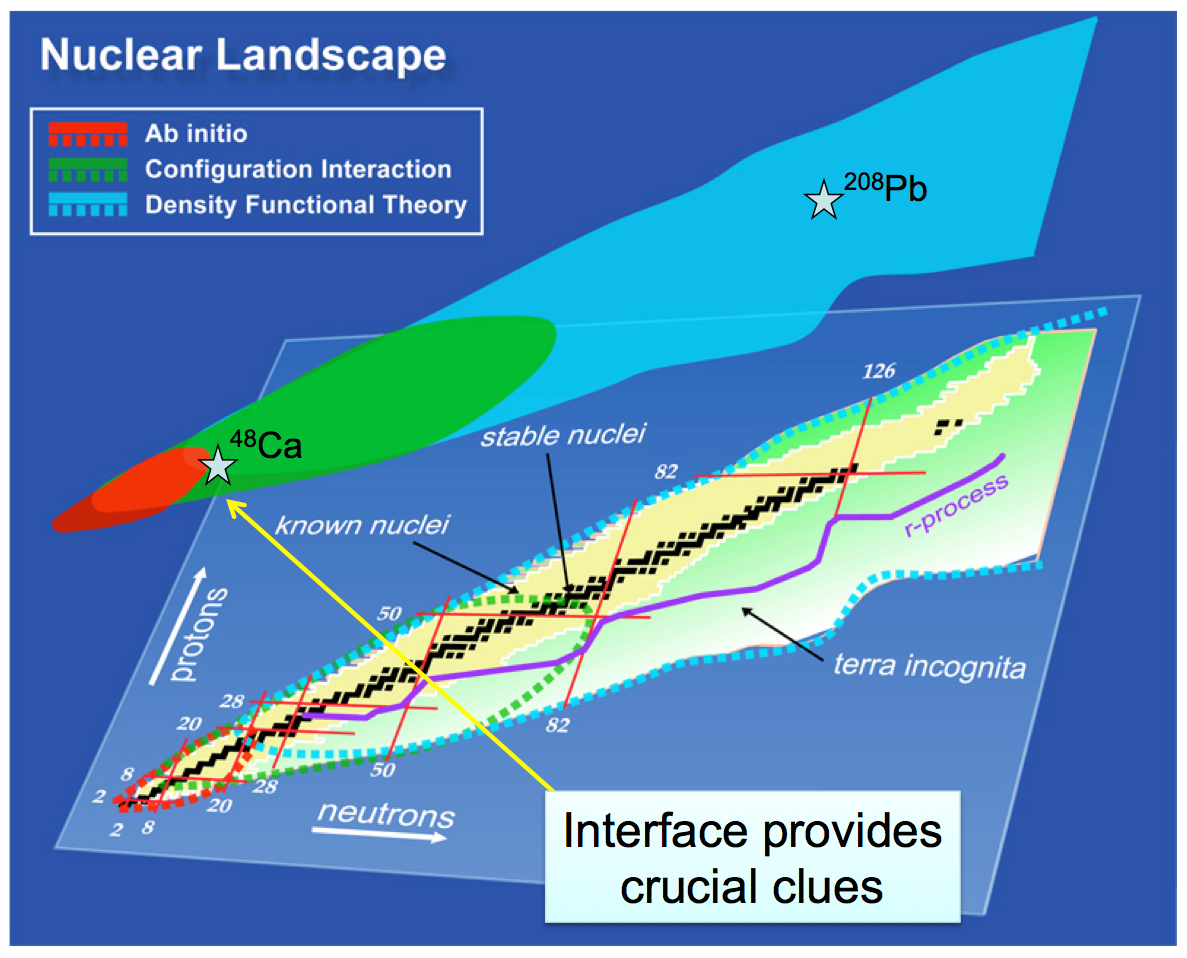
\includegraphics[width=0.5\linewidth]{Nuclear_Landscape}
    \caption{Nuclear Landscape}
    \label{fig:nuclear_landscape}
\end{figure}
As tiny as the neutron skin thickness, to measure it relatively accurately, it is
better to have a thicker neutron skin. So the target element is desired to
have a large neutron excess. Unfortunately, most medium and heavy nuclei that
have extra neutrons are unstable because of those extra neutrons. Only
some nuclei with specific number of protons and neutrons are stable, those specific
numbers are called the magic number. The magic number arises from the nucleon 
shell structure -- when a shell is fully filled and the next higher energy shell 
is empty, and hence it is hard to separate out a nucleon from that closed shell.

Nuclei whose numbers of protons and neutrons are both magic are called doubly
magic nuclei, which are more stable than single magic nuclei. Of all the known
neutron-rich doubly magic nuclei, ${}^{10}$He, ${}^{28}$O, \Ca, ${}^{78}$Ni, 
${}^{132}$Sn and \Pb, \Ca and \Pb are the only two that are stable, hence they
are chosen for PREX-II and CREX.

For double magic nuclei, the energy of the first excited state is much larger 
than that of ground state. The energies needed to excite \Ca and \Pb are 
3.84 and 2.6~MeV respectively. 
Together with the high momentum resolution of our spectrometers, we can easily
separate inelastic scatterings from elastic ones, giving grounds for our choice of
flux integration detection.

Other advantages of \Ca and \Pb include
\begin{itemize}
    \item Both nuclei are spin-0, so that we don't need to worry about the target polarization.
    \item \Pb is heavy while \Ca is moderately heavy. As is discussed in the previous section, 
	the elastic scattering is quasi, not exact. The small energy change is 
	caused by the target recoil. The heavier the target nucleus, the smaller the 
	recoil effect, therefore the better our measurement of $Q^2$ and the 
	scattering angle.
\end{itemize}

Finally, one more reason for the choice of \Ca: \Ca lies in the medium region of the nuclear 
landscape, as shown in Fig.~\ref{fig:nuclear_landscape}. Compared to \Pb, it
is a smaller system that is accessible from ab-initio methods \cite{Hagen2016}.
So it allows direct comparison to Chiral Effective Field Theory (EFT) calculations,
which is very sensitive to three-nucleon forces. In other words, it can be used
to probe three-nucleon forces. On the other hand, it is large enough to apply the
DFT methods. By measuring the neutron skin thickness of \Ca, 
we hope to provide some inputs for bridging these two approaches. 

